\documentclass[11pt,a4paper]{article}
\usepackage[margin=26mm,headheight=15pt]{geometry}
\usepackage[T1]{fontenc}
\usepackage[utf8]{inputenc}
\usepackage{lmodern}
\usepackage{amsmath,amssymb,amsthm,mathtools,mathrsfs}
\usepackage{microtype,booktabs,tabularx,longtable,graphicx,enumitem}
\usepackage{xcolor,fancyhdr,lastpage}
\usepackage[unicode]{hyperref}
\definecolor{navy}{HTML}{19364D}
\definecolor{teal}{HTML}{147D86}
\hypersetup{colorlinks=true,linkcolor=navy,citecolor=navy,urlcolor=teal,
 pdftitle={Harmonic Euler Sums and Lerch Zero Geometry},
 pdfauthor={Research continuation prepared with ChatGPT for ProveIt},
 pdfsubject={Entire continuation, real zeros, diagonal velocities, optimal exterior barriers}}
\urlstyle{same}
\newtheorem{theorem}{Theorem}[section]
\newtheorem{proposition}[theorem]{Proposition}
\newtheorem{lemma}[theorem]{Lemma}
\newtheorem{corollary}[theorem]{Corollary}
\theoremstyle{definition}
\newtheorem{definition}[theorem]{Definition}
\newtheorem{conjecture}[theorem]{Conjecture}
\theoremstyle{remark}
\newtheorem{remark}[theorem]{Remark}
\newcommand{\sech}{\operatorname{sech}}
\newcommand{\csch}{\operatorname{csch}}
\newcommand{\E}{\mathbb E}
\newcommand{\Var}{\operatorname{Var}}
\newcommand{\Cov}{\operatorname{Cov}}
\newcommand{\stirling}[2]{\genfrac{[}{]}{0pt}{}{#1}{#2}}
\numberwithin{equation}{section}
\setlist{leftmargin=*,itemsep=3pt,topsep=5pt}
\setcounter{tocdepth}{2}
\setlength{\emergencystretch}{2em}
\allowdisplaybreaks[1]
\pagestyle{fancy}
\fancyhf{}
\fancyhead[L]{\small\textsc{Harmonic Euler sums and Lerch zero geometry}}
\fancyhead[R]{\small ProveIt research}
\fancyfoot[L]{\small 10 October 2026}
\fancyfoot[R]{\small\thepage\ / \pageref{LastPage}}
\renewcommand{\headrulewidth}{0.3pt}

\title{\vspace{-1.5em}\color{navy}\textbf{Harmonic Euler Sums\\and Lerch Zero Geometry}\\[.65em]
\large Entire Continuation, Infinite Direction Changes,\\
and an Optimal Exterior Barrier}
\author{Research continuation prepared for the ProveIt project}
\date{10 October 2026}

\begin{document}
\maketitle
\thispagestyle{empty}
\begin{abstract}
We continue the ProveIt polylogarithm research in three directions.
First, the odd-denominator harmonic Euler sum
$S(s)=\sum_{n\ge0}(-1)^nH_n(2n+1)^{-s}$ extends to an entire
function with exactly one simple real zero in each interval
$(-2m-1,-2m)$, $m\ge1$, and no other real zeros. A Fourier--beta
identity and a quantitative variance bound prove the classification.
We obtain exact negative-integer evaluations, a complex zero-free
half-plane, monotone real-zero displacements, and all-orders zero
asymptotics.
Second, for the smallest Lerch zero on the diagonal $k=n-1$,
an exact inverse-function generating identity proves infinitely many
positive and infinitely many negative initial velocities, for every
positive lattice spacing. An explicitly labelled complex-singularity
conjecture gives a proposed quantitative refinement.
Third, we solve the incoming exterior-operator optimization problem:
a cubic algebraic number determines the unique optimal constant
coefficient and the least cutoff for the geometric sum. The strict
pointwise problem has the same infimum, but does not attain it.
Convergent coefficient formulas, two-scale cutoff expansions, exact
rational certificates, independent numerical diagnostics, proposed
manuscript corrections, and fourteen further research directions
accompany the proofs.
The already proved $S_4$ reduction is credited to the inspected
baseline; the weight-seven $S_6$ reduction remains open.
\end{abstract}

\vfill
\noindent\textbf{Source baseline.}\quad
\texttt{VladimirReshetnikov/ProveIt}\\
Commit:
\texttt{a0a90ef31877f98be437191c48b46f02d5456867}.

\medskip
\noindent\textbf{Proof standard.}\quad
Ordinary analytic and algebraic proofs, with reproducible finite
certificates. Numerical illustrations are identified as diagnostics;
no proof-assistant verification or exhaustive priority claim is implied.
\clearpage
\begingroup
\small
\tableofcontents
\endgroup
\clearpage
\section{Introduction and the state of the problem}
\label{sec:introduction}

The ProveIt polylogarithm manuscript brings together exact cyclotomic
identities, positive-kernel representations, and zero geometry of
Stieltjes--Lerch derivatives. The most useful next step is to distinguish
questions about a fixed integer weight from questions about an entire
family. A special-value reduction asks which periods suffice to express
one number. An order interpolation asks how those numbers fit into a
holomorphic function. A zero-motion problem asks what remains uniform
when two discrete indices change together. These questions interact, but
a solution to one does not automatically solve the others.

This article develops three results beyond the inspected source baseline.
The proofs are given in full, with classical analytic inputs either
derived here or explicitly identified. The accompanying programs check
finite identities and numerical conventions; the infinite conclusions
do not rest on an integer-relation search or a scan of zeros.

\subsection{The harmonic Euler sum as a function of its order}

Let $H_0=0$ and $H_n=\sum_{j=1}^n j^{-1}$. The manuscript's mixed
Gaussian sums are the positive-integer values of
\[
 S(s)=\sum_{n=0}^{\infty}\frac{(-1)^nH_n}{(2n+1)^s},
 \qquad \Re s>0.
\]
Our first main result is that this function extends to an entire function
whose complete real zero set is
\[
 \{\sigma_m:m\ge1\},\qquad -2m-1<\sigma_m<-2m,
\]
with every zero simple. In particular $S(s)<0$ for real $s\ge-2$.
We also prove that $S$ has no complex zero in $\Re s\ge3$.

The continuation itself is a standard Mellin-regularization argument.
The new work is the global zero classification. A differentiated
Fourier--beta integral gives
\[
 S(-q)=\frac{cD(q)}2\{R(q)\cos(cq)-\sin(cq)\},\qquad c=\frac\pi2,
\]
where $D(q)>0$ and $R$ is a ratio of explicit Mellin moments.
We prove $R(q)>0$ and $0<R'(q)<\pi/2$ for $q\ge2$. This converts
existence and uniqueness in every interval into a strict comparison
with the tangent function. The derivative estimate follows from a
one-dimensional variance inequality and elementary moment bounds.
It covers the first interval as well as the asymptotic regime.

If $N=2m+1$, $\Lambda=\log(N/\pi)+\gamma$, and
$\sigma_m=-N+\varepsilon_m$, then
\[
 \varepsilon_m=
 \frac2\pi\arctan\frac{\pi}{2\Lambda}
 -\frac{\frac12-\frac2\pi\arctan(\pi/(2\Lambda))}
        {N(\Lambda^2+\pi^2/4)}
 +O\!\left(\frac1{N^2\Lambda^2}\right).
\]
We give both a complete expansion in inverse logarithms and a recursive
construction of every correction in $1/N$. Exact negative-integer
identities in generalized secant numbers supply an independent arithmetic
description.

\subsection{Diagonal Lerch zeros do not have an eventual common direction}

For $n\ge0$, $k\ge1$, $h>0$, and $0\le\rho\le1$, define
\[
 \mathscr F_{n,k}^{\rho,h}(a)=
 \sum_{m=0}^{\infty}\rho^m(-1)^{n+k}
 \frac{d^k}{da^k}\left(\frac{\log^n(a+mh)}{a+mh}\right),
 \qquad a>0.
\]
The endpoint $\rho=1$ is defined by this convergent derivative series.
On the diagonal $k=n-1$, the smallest elementary zero is $a=1$.
It continues to an analytic local zero branch $a_n^{(h)}(\rho)$.
For $A=1+h$, put $v_n(A)=(a_n^{(h)})'(0)$.
We prove the exact convergent generating identity
\[
 \sum_{n\ge1}v_n(A)t^n=\log A-u_A(t),\qquad
 e^{u_A(t)}=A+t\,u_A(t),\qquad u_A(0)=\log A.
\]
Here the $n=1$ coefficient is an auxiliary term completing the generating
function; the zero-branch assertion concerns $n\ge2$.

For every real $A>1$, infinitely many $v_n(A)$ are positive and infinitely
many are negative. The proof uses Lagrange inversion and a
positive-coefficient argument: the inverse $u_A$ is analytic along the
whole positive real axis and has unbounded logarithmic growth, which
excludes eventually one-sign Taylor coefficients. This is compatible
with a theorem that fixes $n$ before letting $k$ grow; it shows why that
order of quantifiers matters.

\subsection{An explicit solution to the exterior-operator problem}

For $n\ge2$, set
\[
 g_n(x)=x^{-2}(\log x)^{n-1}(n-\log x),\qquad
 U_n(a,\rho)=\sum_{m\ge0}\rho^m g_n(a+m).
\]
The incoming \emph{Lerch Global Phase} report asks for the best exterior
cutoff obtainable by optimizing the positive constant in
$\partial_a+\lambda$ \cite{IncomingPhase}. Let $r_n$ be the unique
positive root of
\[
 r^3+nr^2-nr-n=0.
\]
The optimal coefficient is
\[
 \lambda_n=(2-r_n)e^{-n-r_n},\qquad 1<r_n<\frac{1+\sqrt5}{2}.
\]
We give a scalar equation uniquely defining the least cutoff $B_n$,
prove
\[
 (\partial_a+\lambda_n)U_n(a,\rho)<0
 \quad(a\ge B_n,\ 0<\rho\le1),
\]
and prove that no smaller cutoff works uniformly over these parameters.
At that cutoff the coefficient is unique. For the corresponding strict
pointwise problem, the same cutoff is an infimum and is not attained:
there is an unavoidable tangency in the negative tail. This boundary
qualification is part of the solution.

The algebraic parameter $r_n$ tends to the golden ratio. Its series in $1/n$ has exact
radius of convergence $5/27$, and the cutoff has explicit exponentially
small corrections in logarithmic coordinates. These are quantitative
identities, rather than numerical fits.

\subsection{Source baseline, attribution, and proof status}
\label{sec:baseline}

The source baseline is the repository commit
\[
 \texttt{a0a90ef31877f98be437191c48b46f02d5456867},
\]
dated 10 October 2026. The focused audit used all forty manuscript chapter
files and the mathematical source material in the sixteen incoming
archives listed in the accompanying provenance record. This is a focused
research audit, not a claim to have independently re-proved every theorem
in those archives.

At this baseline, the mixed Gaussian $S_4$ reduction is already proved
by a convergent octahedral transformation and an exact finite certificate
\cite{ProjectS4}. The $S_2$ companion, the product-matrix rank theorem,
and several low-index Lerch phase results are also already established.
The two displayed $S_6$ baskets are provably equivalent formulations of
one remaining conjecture \cite{ProjectQuotients}. A frozen $S_8$ vector
has already been disproved by an exact interval exclusion
\cite{ProjectDiscovery}. None of those earlier achievements is claimed
as a result of this article.

Analytic continuation of harmonic Euler Dirichlet series has substantial
precedent \cite{BGP}; integer-weight Euler sums and their colored
multiple-zeta representations are also established subjects
\cite{XuWang}. Lagrange inversion, the Pringsheim principle, and the
Brascamp--Lieb inequality are classical \cite{Gessel2016,Flajolet,BL}.
The claims of progress here are relative to the inspected manuscript and
incoming reports. The literature check was targeted and does not establish
global priority for every formula.

The results designated as theorems below have ordinary analytic or
algebraic proofs. Exact rational computations provide additional finite
certificates. Numerical quadrature and high-precision asymptotic
comparisons are labelled diagnostics. The complex-singularity conjecture
is kept separate from the proved infinite sign theorem, and $S_6$ remains
open.

\begin{table}[htbp]
\centering
\small
\begin{tabularx}{\textwidth}{@{}p{.28\textwidth}X p{.19\textwidth}@{}}
\toprule
Question & Result in this article & Status\\
\midrule
Real zeros of $S(s)$ &
Entire continuation; exactly one simple zero in each
$(-2m-1,-2m)$; no other real zeros & Proved\\
Diagonal initial motion &
Exact inverse generating function; infinitely many velocities of each sign
for every $h>0$ & Proved\\
Best constant exterior operator &
Unique optimal coefficient and least uniform summed cutoff;
strict pointwise infimum identified & Proved\\
Quantitative diagonal oscillation &
Candidate accessible conjugate singularities and coefficient asymptotics
& Explicit conjecture\\
Mixed reduction for $S_6$ &
Existing candidate and its two-basket equivalence retained
& Still open\\
\bottomrule
\end{tabularx}
\caption{The principal proof-status distinctions.}
\label{tab:status}
\end{table}

\section{Notation for the order interpolation}
\label{sec:order-notation}

Write $H_0=0$, $H_n=\sum_{j=1}^n1/j$ and
\begin{equation}\label{sorder:def:S}
 S(s)=\sum_{n=0}^{\infty}\frac{(-1)^nH_n}{(2n+1)^s},\qquad \Re s>0.
\end{equation}
Use the positive real logarithm in the denominator, and let
$\beta(s)=\sum_{n\ge0}(-1)^n(2n+1)^{-s}$ denote the Dirichlet beta
function and its entire continuation. Put
\[
 c=\frac\pi2,\qquad G=\beta(2),\qquad
 L(x)=\gamma+\Re\psi\left(\frac{1+ix}{2}\right)\quad(x\ge0).
\]
The gamma logarithmic derivative is $\psi$, and $\gamma=-\psi(1)$.
In particular, $L(0)=-2\log2$.

Analytic continuation of alternating Euler sums and their values at
negative integers belong to an established subject; see
Boyadzhiev--Gadiyar--Padma \cite{BGP}. Our continuation argument is an
elementary instance of that method. The result developed here is the
complete real zero classification for this specific odd-denominator
harmonic interpolation, together with quantitative zero asymptotics.
No exhaustive literature priority claim is made.

\section{Entire continuation and a zero-free real ray}

Define, for $t\ge0$,
\begin{equation}\label{sorder:def:K}
 K(t)=\frac{e^{-t}\log(1+e^{-2t})}{1+e^{-2t}}
     =\frac{\log(2\cosh t)-t}{2\cosh t}.
\end{equation}
The second equality holds on the real line; near zero both sides have
the same analytic germ. The generating function of the harmonic
numbers gives
\[
 -K(t)=\sum_{n\ge0}(-1)^nH_n e^{-(2n+1)t}\qquad(t>0).
\]
Consequently, initially by absolute convergence for $\Re s>1$,
\begin{equation}\label{sorder:eq:Mellin}
 S(s)=-\frac1{\Gamma(s)}\int_0^\infty t^{s-1}K(t)\,dt.
\end{equation}
The original series is locally uniformly convergent for $\Re s>0$:
summation by parts applies because $H_n(2n+1)^{-s}\to0$ and the
successive differences are $O_C(n^{-1-\sigma}\log n)$ on every compact
set $C\subset\{\Re s\ge\sigma>0\}$. Thus \eqref{sorder:eq:Mellin}
represents \eqref{sorder:def:S} throughout that half-plane.

\begin{proposition}\label{sorder:prop:entire}
The function $S$ extends to an entire function, real on the real axis.
For every integer $j\ge0$,
\begin{equation}\label{sorder:eq:negative-derivative}
 S(-j)=(-1)^{j+1}K^{(j)}(0).
\end{equation}
Moreover $S(s)<0$ for every real $s\ge-2$.
\end{proposition}
\begin{proof}
The function $K$ is analytic near zero and is $O(e^{-3t})$ at positive
infinity, as are each of its fixed-order derivatives. Subtract its
Taylor polynomial on $[0,1]$. The Mellin integral then continues
meromorphically across any finite part of the plane, with possible
simple poles at $s=-j$ and residues $K^{(j)}(0)/j!$.
The reciprocal gamma function has a simple zero there with leading
coefficient $(-1)^j j!$. This cancels every pole and gives
\eqref{sorder:eq:negative-derivative}. The construction uses real
Taylor coefficients and a real kernel, proving the reality assertion.

For the sign assertion we show $K''(t)>0$ on $[0,\infty)$. Set
$y=e^{-2t}\in(0,1]$. Direct differentiation gives
\begin{equation}\label{sorder:eq:Ksecond}
 K''(t)=\frac{\sqrt y}{(1+y)^3}
 \left((y^2-6y+1)\log(1+y)-4y^2+8y\right).
\end{equation}
If $y^2-6y+1\ge0$, the bracket is positive. Otherwise
$\log(1+y)<y$, so the bracket is strictly greater than
\[
 (y^2-6y+1)y-4y^2+8y=y(y-1)(y-9)\ge0.
\]
Two integrations by parts in \eqref{sorder:eq:Mellin} give
\begin{equation}\label{sorder:eq:twice-parts}
 S(s)=-\frac1{\Gamma(s+2)}
       \int_0^\infty t^{s+1}K''(t)\,dt,
       \qquad \Re s>-2.
\end{equation}
The integrations are first justified for $\Re s>0$; analyticity then
extends the identity to the stated half-plane. For real $s>-2$ all
factors in the integral and the gamma denominator are positive, so
$S(s)<0$. At the endpoint,
$S(-2)=-K''(0)=(\log2-1)/2<0$.
\end{proof}

\begin{corollary}[A complex zero-free half-plane]\label{sorder:cor:right-half-plane}
For every $s\in\mathbb C$ with $\Re s\ge3$,
\[
 |3^sS(s)+1|<\frac56.
\]
In particular $S$ has no zero in that half-plane.
\end{corollary}
\begin{proof}
The $n=1$ term of $3^sS(s)$ is $-1$, and absolute convergence gives
\[
 |3^sS(s)+1|\le27\sum_{n=2}^\infty\frac{H_n}{(2n+1)^3}.
\]
For $n\ge6$, use $H_n\le1+\log n$ and
$(2n+1)^3>8n^3$. The function $(1+\log x)x^{-3}$ decreases for
$x\ge5$, so the tail from $n=6$ is at most
$(3+2\log5)/800<7/800$. Therefore
\[
 \sum_{n=2}^\infty\frac{H_n}{(2n+1)^3}
 <\sum_{n=2}^5\frac{H_n}{(2n+1)^3}+\frac7{800}
 =\frac{122481517493}{3993750684000}.
\]
Multiplication by $27$ gives a rational number strictly below $5/6$.
\end{proof}

\subsection{Exact values at the negative integers}

Define the generalized secant numbers by
\[
 (\sec z)^\alpha=\sum_{m\ge0}E_{2m}(\alpha)\frac{z^{2m}}{(2m)!},
 \qquad E_{2m}=E_{2m}(1)>0.
\]
A prime on $E_{2m}(\alpha)$ will mean differentiation with respect
to $\alpha$. Comparison of the even and odd parts of \eqref{sorder:def:K}
gives the following exact formulas.
\begin{corollary}\label{sorder:cor:negative-values}
For $m\ge0$,
\begin{align}
 S(-2m)&=\frac{(-1)^m}{2}
       \left(E'_{2m}(1)-E_{2m}\log2\right),\label{sorder:eq:negative-even}\\
 S(-2m-1)&=\frac{(-1)^{m+1}}2(2m+1)E_{2m}.
 \label{sorder:eq:negative-odd}
\end{align}
For $m\ge1$, $(-1)^mS(-2m)>0$.
\end{corollary}
\begin{proof}
The even part of $K$ is
$\tfrac12\sech t\,[\log2+\log\cosh t]$ and its odd part is
$-\tfrac12t\sech t$. Use
$\partial_\alpha(\sech t)^\alpha|_{\alpha=1}
=-\sech t\log\cosh t$ and $\sech t=\sec(it)$ in
\eqref{sorder:eq:negative-derivative}. This proves both identities.
The Taylor coefficients of $\log\sec z$ in positive even degrees are
positive: its derivative is $\tan z$, whose positive coefficients
follow recursively from $u'=1+u^2$, $u(0)=0$.
Therefore, when $m\ge1$, $E_{2m}(\alpha)$ is a nonzero polynomial
in positive powers of $\alpha$ with nonnegative coefficients.
It follows that $E'_{2m}(1)\ge E_{2m}$, proving the sign because
$\log2<1$.
\end{proof}
For example,
\[
\begin{array}{c|rrrrrrr}
 s&0&-1&-2&-3&-4&-5&-6\\\hline
 S(s)&-\frac{\log2}{2}&-\frac12&\frac{\log2-1}{2}&\frac32&
 4-\frac52\log2&-\frac{25}2&\frac{61\log2-121}{2}
\end{array}
\]
The sign change between $-2m-1$ and $-2m$ already proves the existence
of at least one zero in each interval. It gives neither uniqueness nor
exclusion of other real zeros; those require the next argument.

\section{A Fourier--beta identity}

For real $\alpha>0$ define
\[
 B_\alpha(s)=\frac1{\Gamma(s)}\int_0^\infty
        \frac{t^{s-1}}{(2\cosh t)^\alpha}\,dt,
 \qquad\Re s>0.
\]
In particular $B_1(s)=\beta(s)$. From the kernels, or from the
binomial series and $(\alpha)_n$ differentiated at $\alpha=1$,
\begin{equation}\label{sorder:eq:parameter-derivative}
 S(s)=s\beta(s+1)+\left.\partial_\alpha B_\alpha(s)\right|_{\alpha=1}.
\end{equation}
This identity extends wherever its two sides are continued.

\begin{lemma}\label{sorder:lem:Fourier}
For $\Re s<1$,
\begin{equation}\label{sorder:eq:Fourier-B}
 B_\alpha(s)=\frac{\cos(\pi s/2)}{2\pi\Gamma(\alpha)}
 \int_0^\infty x^{-s}
 \Gamma\left(\frac{\alpha+ix}{2}\right)
 \Gamma\left(\frac{\alpha-ix}{2}\right)\,dx.
\end{equation}
On the left this means analytic continuation. Differentiation with
respect to $\alpha$ is valid locally uniformly near $\alpha=1$.
\end{lemma}
\begin{proof}
The substitution $u=e^{2t}$ and the beta integral show
\[
 \int_{-\infty}^\infty\frac{e^{ixt}}{(2\cosh t)^\alpha}\,dt
 =\frac{\Gamma((\alpha+ix)/2)\Gamma((\alpha-ix)/2)}{2\Gamma(\alpha)}.
\]
Fourier inversion and the Mellin transform of the cosine prove
\eqref{sorder:eq:Fourier-B} first in $0<\Re s<1$. For a direct
justification of the interchange, insert $e^{-\varepsilon t}$ before
the Mellin integral, integrate in $t$, and then send
$\varepsilon\downarrow0$. The resulting kernels are bounded near
zero by a constant times $x^{-\Re s}$, and the gamma product decays
exponentially at infinity. Dominated convergence applies.
The right side is holomorphic in $\Re s<1$, so it supplies the
claimed continuation. Differentiation in $\alpha$ only introduces
digamma factors growing logarithmically at infinity; the same
domination applies on a compact positive $\alpha$-interval.
\end{proof}

For real $q>0$ put
\begin{align}
 J(q)&=\int_0^\infty x^q\sech(cx)\,dx,
 \label{sorder:def:J}\\
 A(q)&=\int_0^\infty x^q\sech(cx)L(x)\,dx,
 \label{sorder:def:A}\\
 D(q)&=\int_0^\infty x^q\sech(cx)\tanh(cx)\,dx,
 \label{sorder:def:D}\\
 R(q)&=\frac{A(q)}{cD(q)}.
 \label{sorder:def:R}
\end{align}
The letter $D$ here denotes a positive integral, not differentiation.

\begin{proposition}\label{sorder:prop:reflected}
For $q>0$,
\begin{equation}\label{sorder:eq:reflected}
 S(-q)=\frac{cD(q)}2
       \left(R(q)\cos(cq)-\sin(cq)\right).
\end{equation}
Moreover,
\begin{equation}\label{sorder:eq:moments}
 J(q)=2\Gamma(q+1)c^{-q-1}\beta(q+1),\qquad
 D(q)=\frac q c J(q-1).
\end{equation}
\end{proposition}
\begin{proof}
At $\alpha=1$ the reflection formula gives
$\Gamma((1+ix)/2)\Gamma((1-ix)/2)=\pi\sech(cx)$.
The logarithmic $\alpha$ derivative of the full gamma quotient in
\eqref{sorder:eq:Fourier-B} is $L(x)$.
Thus the derivative term in \eqref{sorder:eq:parameter-derivative}
at $s=-q$ is $\tfrac12\cos(cq)A(q)$.
Applying the same Fourier formula to $\beta(1-q)$ gives
$\beta(1-q)=\tfrac12\sin(cq)J(q-1)$.
Since $D(q)=qJ(q-1)/c$ by integration by parts, the remaining term is
$-\tfrac12 c\sin(cq)D(q)$. This proves \eqref{sorder:eq:reflected}.
The expansion $\sech(cx)=2\sum_{n\ge0}(-1)^ne^{-(2n+1)cx}$
gives the stated formula for $J(q)$ for $q>0$ by absolute integration.
The integration-by-parts identity for $D$ is valid for every $q>0$.
\end{proof}

\section{The derivative bound that forces uniqueness}

The next estimate is the central analytic input. Its numerical constant
is deliberately coarse; it is small enough for the tangent comparison
and needs no numerical certification.

\begin{lemma}\label{sorder:lem:r}
Let $r(x)=L(x)\coth(cx)/c$ for $x>0$. Then
\begin{equation}\label{sorder:eq:r-derivative}
 0<xr'(x)\le a+\frac b x,\qquad
 a=\frac2c=\frac4\pi,\qquad
 b=\frac{2+2\log2}{c^2}.
\end{equation}
\end{lemma}
\begin{proof}
The digamma series gives
\begin{align}
 L(x)&=-2\log2+2\sum_{\substack{k\ge1\\k\text{ odd}}}
          \frac{x^2}{k(k^2+x^2)},\label{sorder:eq:L-series}\\
 L'(x)&=4x\sum_{\substack{k\ge1\\k\text{ odd}}}
          \frac{k}{(k^2+x^2)^2}>0.\label{sorder:eq:L-prime}
\end{align}
These series converge locally uniformly in $x$. Also
\[
 L'(x)=\int_0^\infty\frac{u\sin(xu)}{\sinh u}\,du.
\]
Writing $h(u)=u/\sinh u$, integration by parts yields
\[
 xL'(x)=1+\int_0^\infty h'(u)\cos(xu)\,du.
\]
Here $h$ decreases from $1$ to $0$, so
$\int_0^\infty|h'(u)|\,du=1$ and $0<xL'(x)\le2$.

Now
\[
 r'(x)=\frac{L'(x)}c\coth(cx)-L(x)\csch^2(cx).
\]
This is positive whenever $L(x)\le0$. If $L(x)>0$, comparison term
by term in \eqref{sorder:eq:L-series}--\eqref{sorder:eq:L-prime}
gives
\[
 L(x)<L(x)+2\log2\le\frac{1+x^2}{2}\,xL'(x).
\]
It follows that
\[
 r'(x)>\frac{L'(x)}c\coth(cx)
 \left(1-\frac{cx(1+x^2)}{\sinh(2cx)}\right)>0.
\]
The last inequality follows from
$\sinh(\pi x)\ge\pi x+(\pi x)^3/6>cx(1+x^2)$.
Finally $L(x)\ge-2\log2$, $\coth y\le1+1/y$ and $\sinh y\ge y$
give
\[
 xr'(x)\le\frac2c\left(1+\frac1{cx}\right)
       +\frac{2\log2}{c^2x},
\]
which is \eqref{sorder:eq:r-derivative}.
\end{proof}

For completeness we give the needed one-dimensional form of the
Brascamp--Lieb variance inequality \cite{BL}.
\begin{lemma}\label{sorder:lem:BL}
For a probability density proportional to $e^{-V(x)}$ on an interval,
with $V''(x)>0$,
\[
 \Var(f)\le\E\frac{f'(x)^2}{V''(x)}.
\]
Consequently
$|\Cov(f,g)|^2\le
\E(f'^2/V'')\E(g'^2/V'')$ whenever the displayed quantities exist.
\end{lemma}
\begin{proof}
It suffices first to work on a compact interval $[a,b]$ and subtract
the mean of $f$. Put
$u(x)=e^{V(x)}\int_a^x f(t)e^{-V(t)}\,dt$.
Then $u(a)=u(b)=0$ and $f=u'-V'u$. Integration by parts gives
\[
 \E f^2=-\E(f'u),\qquad
 \E f^2=\E u'^2+\E(V''u^2).
\]
Cauchy--Schwarz with weights $V''$ implies
$(\E f^2)^2\le\E(f'^2/V'')\E(V''u^2)
\le\E(f'^2/V'')\E f^2$. Division proves the variance bound.
Exhaust the original interval by compact intervals and use truncation
and convergence of the stated integrals. The covariance assertion
then follows from Cauchy--Schwarz and the two variance bounds.
\end{proof}

\begin{theorem}\label{sorder:thm:R}
For every real $q\ge2$,
\begin{equation}\label{sorder:eq:R-bound}
 R(q)>0,\qquad
 0<R'(q)<\frac1q\sqrt{\frac{181}{27}}<\frac\pi2.
\end{equation}
\end{theorem}
\begin{proof}
Give $(0,\infty)$ the probability density
\[
 d\nu_q(x)=\frac{x^q\sech(cx)\tanh(cx)}{D(q)}\,dx.
\]
Then $R(q)=\E_{\nu_q}r(X)$ and differentiation in $q$ gives
$R'(q)=\Cov_{\nu_q}(r(X),\log X)>0$, because both functions are
strictly increasing and the density has full support. Differentiation
is justified by absolute integrability of the additional logarithm.
Since $S(-2)=(\log2-1)/2$, \eqref{sorder:eq:reflected} gives
$A(2)=1-\log2>0$, whence $R(2)>0$ and $R(q)>0$ for all $q\ge2$.

The negative logarithm of the density, up to a constant, is
\[
 V_q(x)=-q\log x+\log\cosh(cx)-\log\tanh(cx).
\]
Its second derivative is
\[
 V_q''(x)=\frac q{x^2}+c^2\sech^2(cx)
     +4c^2\frac{\cosh(2cx)}{\sinh^2(2cx)}\ge\frac q{x^2}.
\]
Lemma~\ref{sorder:lem:BL}, applied to $r$ and $\log x$, therefore yields
\begin{equation}\label{sorder:eq:covariance-bound}
 R'(q)\le\frac1q\sqrt{\E_{\nu_q}(Xr'(X))^2}.
\end{equation}
There is no endpoint assumption hidden here: as $x\downarrow0$,
$r(x)=O(x^{-1})$, $xr'(x)=O(x^{-1})$, and the density is
$O(x^{q+1})$. All second moments and energy integrals used in the
lemma are finite for $q\ge2$. The tails are exponentially integrable.

For $j=1,2$, $\E_{\nu_q}X^{-j}$ decreases with $q$ by the same
covariance differentiation, now applied to a decreasing function and
$\log x$. At $q=2$ the two inverse moments coincide. Indeed,
\[
 D(0)=\frac1c,\quad D(1)=\frac1c,\quad D(2)=\frac{4G}{c^3},
\]
so
\[
 \E_{\nu_q}X^{-1},\ \E_{\nu_q}X^{-2}
 \le\mu:=\frac{\pi^2}{16G}<\frac34.
\]
Here $G>1-1/9=8/9$ by the alternating-series estimate and
$\pi^2<10$, so even $\mu<45/64$ suffices. The elementary inequalities
$\pi>3$ and $\log2<3/4$ give $a<4/3$ and $b<14/9$ in
Lemma~\ref{sorder:lem:r}. Consequently
\[
 \E_{\nu_q}(Xr'(X))^2
 \le a^2+2ab\mu+b^2\mu
 <\frac{16}{9}+\frac{28}{9}+\frac{49}{27}
 =\frac{181}{27}.
\]
This proves the first derivative bound. For $q\ge2$ its square is
at most $181/108<9/4<c^2$, proving the final strict inequality.
\end{proof}

\section{Complete classification of the real zeros}

\begin{theorem}\label{sorder:thm:all-real-zeros}
For each integer $m\ge1$, $S$ has exactly one real zero
\[
 \sigma_m\in(-2m-1,-2m).
\]
Every such zero is simple. These are all the real zeros of $S$.
The displacements $\varepsilon_m=\sigma_m+2m+1$ strictly decrease
with $m$. In particular, $\sigma_m-\sigma_{m+1}>2$.
\end{theorem}
\begin{proof}
There are no zeros on $[-2,\infty)$ by
Proposition~\ref{sorder:prop:entire}. Write $q=-s>2$.
On $(2m,2m+1)$, equation \eqref{sorder:eq:reflected} is equivalent to
\[
 \tan(c(q-2m))=R(q).
\]
The left side increases from $0$ to $+\infty$. The right side is
positive and finite, and the derivative of their difference is
$c\sec^2(c(q-2m))-R'(q)>0$ by Theorem~\ref{sorder:thm:R}.
There is therefore exactly one solution. At that solution the same
strict inequality and $\cos(cq)\ne0$ show that the derivative of
$S(-q)$ is nonzero, proving simplicity.

On $(2m+1,2m+2)$, $\cos(cq)$ and $-\sin(cq)$ have the same sign.
Since $R(q)>0$ and $D(q)>0$, \eqref{sorder:eq:reflected} cannot vanish.
At the integer endpoints one of the sine and cosine is zero and the
other is nonzero, while $R,D>0$. This exhausts $q>2$.

For the monotonicity write $q_m=2m+\delta_m$, where
$\delta_m\in(0,1)$ and $\tan(c\delta_m)=R(2m+\delta_m)$.
Increasing $m$ strictly increases the right side at every fixed
$\delta$. Since the difference between the left and right sides is
strictly increasing in $\delta$, its unique zero moves to the right.
Thus $\delta_{m+1}>\delta_m$, or
$\varepsilon_{m+1}<\varepsilon_m$, as claimed.
\end{proof}

\section{All-orders asymptotics of the zero displacement}

For $k\ge1$ define
\[
 d_k=\frac{(-1)^{k+1}2^{2k}B_{2k}(1/2)}{2k},
 \quad d_1=-\frac16,\quad d_2=-\frac7{60},\quad d_3=-\frac{31}{126}.
\]
Here $B_n(x)$ is the Bernoulli polynomial. Let
$q^{\underline j}=q(q-1)\cdots(q-j+1)$.

\begin{lemma}\label{sorder:lem:R-asymptotic}
For every fixed integer $K\ge1$, as real $q\to+\infty$,
\begin{equation}\label{sorder:eq:R-asymptotic}
 cR(q)=\psi(q+1)+\gamma-\log\pi
       +\sum_{k=1}^{K-1}\frac{d_kc^{2k}}{q^{\underline{2k}}}
       +O_K(q^{-2K}).
\end{equation}
In particular,
\begin{equation}\label{sorder:eq:R-first}
 cR(q)=\log(q/\pi)+\gamma+\frac1{2q}
                  -\frac{2+\pi^2}{24q^2}+O(q^{-3}).
\end{equation}
\end{lemma}
\begin{proof}
The ordinary sectorial digamma expansion \cite[\S5.11]{DLMF}, applied on the vertical
line with real part $1/2$, gives
\[
 L(x)=\gamma+\log(x/2)+\sum_{k=1}^{K-1}d_kx^{-2k}
                     +O_K(x^{-2K})\qquad(x\to\infty).
\]
The coefficient formula follows either from the shifted Bernoulli
expansion of $\psi(z+1/2)$ or by expanding the ordinary formula in
$1/(ix/2)$. The error may be bounded globally by $C_Kx^{-2K}$ for
all $x>0$: on $(0,1]$ the actual function $L$ is bounded, and each
subtracted power and logarithm is bounded by a constant times
$x^{-2K}$. Hence for $q>2K-1$,
\[
 A(q)=J'(q)+(\gamma-\log2)J(q)
       +\sum_{k=1}^{K-1}d_kJ(q-2k)+O_K(J(q-2K)).
\]
Use \eqref{sorder:eq:moments}. The first quotient, multiplied by $c$,
is
\[
 \frac{\beta(q+1)}{\beta(q)}
 \left(\psi(q+1)+\gamma-\log\pi+
                         \frac{\beta'(q+1)}{\beta(q+1)}\right).
\]
The $k$th remaining quotient is
$d_kc^{2k}\beta(q-2k+1)/(q^{\underline{2k}}\beta(q))$.
For fixed shifts, the beta ratios are $1+O_K(3^{-q})$, and the
logarithmic derivative is $O_K(3^{-q})$, directly from their
absolutely convergent Dirichlet series. The integrated error divided
by $qJ(q-1)/c$ is $O_K(q^{-2K})$. This proves
\eqref{sorder:eq:R-asymptotic}; expanding $\psi(q+1)$ gives
\eqref{sorder:eq:R-first}.
\end{proof}

\begin{theorem}\label{sorder:thm:zero-asymptotic}
Write
\[
 N=2m+1,\quad \sigma_m=-N+\varepsilon_m,\quad
 \Lambda=\log(N/\pi)+\gamma,\quad Q=\Lambda^2+c^2,
 \quad e_0=\frac1c\arctan\frac c\Lambda.
\]
Then $0<\varepsilon_m<1$ and
\begin{equation}\label{sorder:eq:zero-two-scales}
 \varepsilon_m=e_0-
       \frac{\tfrac12-e_0}{NQ}
       +O\left(\frac1{N^2\Lambda^2}\right)
       \qquad(m\to\infty).
\end{equation}
For every fixed $K\ge1$,
\begin{equation}\label{sorder:eq:zero-log-series}
 \varepsilon_m=
 \sum_{j=0}^{K-1}\frac{(-1)^jc^{2j}}{(2j+1)\Lambda^{2j+1}}
       +O_K(\Lambda^{-2K-1}).
\end{equation}
Thus the first three logarithmic terms are
$\Lambda^{-1}-\pi^2/(12\Lambda^3)+\pi^4/(80\Lambda^5)$.
The consecutive-zero gaps satisfy
\begin{equation}\label{sorder:eq:zero-gaps}
 \sigma_m-\sigma_{m+1}
 =2+\frac{2}{N(\Lambda^2+c^2)}
       +O\left(\frac1{N^2\Lambda^2}\right).
\end{equation}
\end{theorem}
\begin{proof}
The exact zero equation is
\begin{equation}\label{sorder:eq:epsilon-equation}
 c\cot(c\varepsilon_m)=cR(N-\varepsilon_m).
\end{equation}
Lemma~\ref{sorder:lem:R-asymptotic}, uniformly for $0\le\varepsilon\le1$,
gives
\[
 cR(N-\varepsilon)
 =\Lambda+\frac{\tfrac12-\varepsilon}{N}+O(N^{-2}).
\]
The solution of $c\cot(ce_0)=\Lambda$ is the stated $e_0$ for all
sufficiently large $N$. The right side of the preceding estimate
shows that the left side at $\varepsilon_m$ differs from $\Lambda$
by $O(N^{-1})$. Its inverse has derivative
$-1/(\Lambda^2+c^2)$ at $\Lambda$, so
$\varepsilon_m-e_0=O(N^{-1}\Lambda^{-2})$.
Taylor expansion of the left side about $e_0$, whose first derivative
is $-Q$ and second derivative is $2Q\Lambda$, now yields
\[
 -Q(\varepsilon_m-e_0)
 =\frac{\tfrac12-e_0}{N}+O(N^{-2}).
\]
The quadratic error is $O(N^{-2}/\Lambda)$ and is absorbed in the
displayed bound; the displacement inside the right side is even
smaller. Division by $Q$ proves \eqref{sorder:eq:zero-two-scales}.
Finally expand the arctangent. Its Taylor remainder gives the error
in \eqref{sorder:eq:zero-log-series}, while the inverse-index correction
is smaller than every fixed power of $1/\Lambda$.
For \eqref{sorder:eq:zero-gaps}, regard the displayed approximation
as a smooth function of real $N$. Its leading term has derivative
$e_0'(N)=-1/(N(\Lambda^2+c^2))$, and the derivative of the explicit
inverse-index correction is $O(N^{-2}\Lambda^{-2})$.
Take the difference at $N$ and $N+2$ in
\eqref{sorder:eq:zero-two-scales}; its two remainder values have the
same $O(N^{-2}\Lambda^{-2})$ bound.
\end{proof}

\paragraph{An algorithm for every inverse-index correction.}
Equation \eqref{sorder:eq:R-asymptotic} supplies a full expansion in
$1/q$. Substituting
$\varepsilon=e_0+\sum_{j\ge1}a_j(\Lambda)N^{-j}$ into
\eqref{sorder:eq:epsilon-equation} and comparing coefficients determines
$a_j$ recursively: the coefficient of the new unknown is always
$-Q\ne0$. The functions $a_j$ belong to
$\mathbb Q[c^2,\Lambda,e_0,Q^{-1}]$, with Bernoulli numbers as rational
coefficients, and $a_j=O_j(\Lambda^{-2})$.
For each fixed $J\ge1$ the truncation through $a_{J-1}N^{1-J}$ has
error $O_J(N^{-J}\Lambda^{-2})$. To justify this statement, first use
the full remainder in \eqref{sorder:eq:R-asymptotic} to bound the
residual after any fixed formal substitution by $O_J(N^{-J})$.
Derivatives of $c\cot(c\varepsilon)$ at $e_0$ are polynomials in
$\Lambda,c^2$ of degree at most the derivative order plus one.
Induction then gives $a_j=O_j(\Lambda^{-2})$ and controls all Taylor
remainders. The derivative of the exact implicit equation has magnitude
comparable to $Q$, by \eqref{sorder:eq:R-bound} and
$\varepsilon\asymp1/\Lambda$. The mean value theorem divides the
residual by $Q$, proving the stated error. This is an asymptotic
recursion; no convergence of the resulting infinite formal series is asserted.


\section{A diagonal zero branch and infinitely many initial directions}
\label{diag:sec:main}

The fixed-index monotonicity theorem permits its derivative-order threshold
to depend on the Laurent index.  That dependence is essential.  We prove
that on the diagonal $k=n-1$, the smallest zero issuing from the elementary
endpoint moves initially to the right for infinitely many $n$ and initially
to the left for infinitely many $n$.  An exact inverse-function identity
organizes all these velocities.  The result concerns the central elementary
zero at $a=1$, which is separate from the branches near positive Bessel zeros
in the earlier adjacent-index expansion.

\subsection{The shifted lattice and its elementary endpoint}
\label{diag:subsec:lattice}

It is useful to allow an arbitrary lattice spacing $h>0$.  For integers
$n\geq0$, $k\geq1$, define
\begin{equation}\label{diag:eq:f}
 f_{n,k}(a)=(-1)^{n+k}\frac{d^k}{da^k}
                 \left(\frac{\log^n a}{a}\right),\qquad a>0,
\end{equation}
and
\begin{equation}\label{diag:eq:lattice}
 \mathscr F_{n,k}^{\rho,h}(a)
       =\sum_{m=0}^{\infty}\rho^m f_{n,k}(a+mh),
       \qquad 0\leq\rho\leq1.
\end{equation}
At $h=1$ this is the normalized Stieltjes--Lerch derivative family used in
the manuscript.  For $\rho<1$ it is $(-1)^{n+k}$ times the $k$th derivative
of the corresponding logarithmic Lerch series.  At $\rho=1$ we use
\eqref{diag:eq:lattice} itself; the undifferentiated logarithmic series need
not converge.  The derivative series converges absolutely because
\[
 f_{n,k}(x)=O_{n,k}\bigl(x^{-k-1}(1+\log^n x)\bigr)
 \quad(x\longrightarrow\infty).
\]
The convergence is locally uniform in $a>0$, together with any fixed
number of $a$-derivatives.  Near $\rho=0$ the series is jointly holomorphic
in $a$ and $\rho$, using the logarithm analytic near the positive axis.

The elementary polynomial is
\begin{equation}\label{diag:eq:P}
 P_{n,k}(x)=n![z^n]e^{xz}\prod_{j=1}^{k}\left(1+\frac zj\right).
\end{equation}
Differentiating $a^{-1-z}$ and comparing coefficients gives
\begin{equation}\label{diag:eq:elementary}
 f_{n,k}(a)=k!a^{-k-1}P_{n,k}(-\log a).
\end{equation}

\begin{lemma}[The central diagonal zero]\label{diag:lem:central}
For every $n\geq2$, $f_{n,n-1}$ has exactly $n$ simple positive zeros.
Its smallest zero is $1$, and
\begin{equation}\label{diag:eq:central-derivative}
 f_{n,n-1}'(1)=-n!.
\end{equation}
For every $h>0$ there is an $\epsilon_{n,h}>0$ such that
$\mathscr F_{n,n-1}^{\rho,h}$ has exactly $n$ simple positive zeros for
$0\leq\rho<\epsilon_{n,h}$.  Its smallest zero is a real analytic branch
$a_n^{(h)}(\rho)$ with $a_n^{(h)}(0)=1$.
\end{lemma}

\begin{proof}
The polynomial in \eqref{diag:eq:P} is obtained from $x^n$ by applying
$k$ operators $1+\partial_x/j$.  If a real-rooted polynomial $p$ has
distinct roots $r_i$ of multiplicities $m_i$, then away from these roots
the zeros of $p+cp'$, $c>0$, solve
\[
 \frac{p'(x)}{p(x)}=\sum_i\frac{m_i}{x-r_i}=-\frac1c.
\]
The left side is strictly decreasing on each complementary interval.
There is one new simple root between consecutive distinct roots and one
to the left of the smallest root.  An inherited root of multiplicity
$m_i\geq2$ has multiplicity $m_i-1$.  Starting from $x^n$, after $n-1$
operators all $n$ roots are simple; zero is the largest and the others
are negative.  Equation~\eqref{diag:eq:elementary} proves the first claim.

Since $n+(n-1)$ is odd,
\[
 f_{n,n-1}(a)=-\frac{d^{n-1}}{da^{n-1}}
                       \left(\frac{\log^n a}{a}\right).
\]
The expansion $\log^n a/a=(a-1)^n+O((a-1)^{n+1})$ proves
\eqref{diag:eq:central-derivative}.  The analytic implicit function theorem
therefore continues this zero, as well as each of the other simple zeros.

For completeness, no additional positive zeros enter from an endpoint.
For sufficiently large $a$, every term $f_{n,n-1}(a+mh)$ has the same
strict sign, because its argument exceeds the largest elementary zero.
As $a\downarrow0$, the $m=0$ term tends to $+\infty$, while the sum over
$m\geq1$ is bounded uniformly for $a$ in a small positive interval and
$0\leq\rho\leq1$.  Thus there are no zeros sufficiently close to zero.
On the remaining compact set outside small neighborhoods of the elementary
zeros, uniform convergence to $f_{n,n-1}$ as $\rho\downarrow0$ excludes
zeros.  Inside each neighborhood, uniform convergence of the first
$a$-derivative preserves its strict sign and hence gives exactly one
simple zero.  The branch issuing from $1$ is consequently the smallest.
\end{proof}

\subsection{An inverse function generates every diagonal velocity}
\label{diag:subsec:inverse}

Let $\stirling{n}{j}$ denote the unsigned Stirling numbers of the
first kind, fixed by
\[
 \prod_{r=0}^{n-1}(z+r)=\sum_{j=0}^n\stirling{n}{j}z^j.
\]

\begin{theorem}[Exact velocity identity]\label{diag:thm:generator}
For $A>1$ and $n\geq1$, put
\begin{align}
 v_n(A)
  &=-\frac1{n!}\left.\frac{d^{n-1}}{dx^{n-1}}
                  \left(\frac{\log^n x}{x}\right)\right|_{x=A}
                  \label{diag:eq:velocity-derivative}\\
  &=A^{-n}\sum_{j=1}^n
       \stirling{n}{n-j+1}\frac{(-\log A)^j}{j!}.
                  \label{diag:eq:velocity-stirling}
\end{align}
For the lattice spacing $h=A-1$, the smallest diagonal branch satisfies
\begin{equation}\label{diag:eq:root-velocity}
 \bigl(a_n^{(h)}\bigr)'(0)=v_n(A),\qquad n\geq2.
\end{equation}
There is a unique analytic germ $u_A(t)$ at zero satisfying
\begin{equation}\label{diag:eq:inverse-equation}
 e^{u_A(t)}=A+t u_A(t),\qquad u_A(0)=\log A.
\end{equation}
Its coefficients give the convergent ordinary generating identity
\begin{equation}\label{diag:eq:velocity-generator}
 V_A(t):=\sum_{n=1}^{\infty}v_n(A)t^n=\log A-u_A(t)
\end{equation}
for all sufficiently small complex $t$.
\end{theorem}

\begin{proof}
Differentiate the zero equation at $\rho=0$.  The shifted series and
\eqref{diag:eq:central-derivative} give
\[
 \bigl(a_n^{(h)}\bigr)'(0)
   =-\frac{f_{n,n-1}(1+h)}{f_{n,n-1}'(1)}
   =\frac{f_{n,n-1}(A)}{n!},
\]
which is \eqref{diag:eq:velocity-derivative}.  The Stirling identity implies
\[
 P_{n,n-1}(x)
       =n\sum_{j=1}^n\stirling{n}{n-j+1}\frac{x^j}{j!}.
\]
Together with \eqref{diag:eq:elementary}, this proves
\eqref{diag:eq:velocity-stirling}.  The same finite identity holds at $n=1$
by direct calculation; that term is included for the generating function.

Let $y(t)$ solve $y=A+t\log y$, with $y(0)=A$.  The analytic implicit
function theorem supplies a unique germ.  The Lagrange--B\"urmann formula
with outer function $\log y$ gives
\[
 [t^n]\log y(t)
   =\frac1{n!}\left.\frac{d^{n-1}}{dx^{n-1}}
                        \left(\frac{\log^n x}{x}\right)\right|_{x=A}.
\]
This is the standard analytic form of Lagrange inversion
\cite{Gessel2016}.  Set $u_A=\log y$.  Its equation is
\eqref{diag:eq:inverse-equation}, and coefficient comparison proves
\eqref{diag:eq:velocity-generator}.
\end{proof}

\begin{corollary}[An exact quadratic recurrence]\label{diag:cor:recurrence}
Write $L=\log A$ and $p_n(L)=A^n v_n(A)$.  Then $p_1(L)=-L$, and for
$n\geq1$,
\begin{equation}\label{diag:eq:recurrence}
 (n+1)p_{n+1}(L)
   =(n+1-nL)p_n(L)
       +\frac n2\sum_{j=1}^{n-1}p_j(L)p_{n-j}(L).
\end{equation}
Each $p_n$ is a rational polynomial of degree $n$, with constant term zero,
linear coefficient $-1$, and leading coefficient $(-1)^n/n$.
\end{corollary}

\begin{proof}
The generating identity is equivalent to
\[
 A e^{-V_A(t)}=A+t(L-V_A(t)).
\]
Differentiation and elimination of the exponential yield
\begin{equation}\label{diag:eq:ode}
 \bigl(A+t(L-1-V_A(t))\bigr)V_A'(t)=V_A(t)-L.
\end{equation}
The constant coefficient gives $v_1=-L/A$.  At degree $n\geq1$, the
convolution is
\[
 \sum_{j=1}^{n-1}(n-j)v_jv_{n-j}
       =\frac n2\sum_{j=1}^{n-1}v_jv_{n-j}.
\]
Multiplication by $A^n$ gives \eqref{diag:eq:recurrence}.  The coefficient
statements follow directly from \eqref{diag:eq:velocity-stirling}, using
$\stirling{n}{n}=1$ and
$\stirling{n}{1}=(n-1)!$.
\end{proof}

\begin{corollary}[Nonvanishing at algebraic lattice endpoints]
\label{diag:cor:algebraic-nonvanishing}
If $A>1$ is algebraic, then $v_n(A)\ne0$ for every $n\ge1$.
\end{corollary}
\begin{proof}
The Hermite--Lindemann theorem implies that $\log A$ is transcendental:
it is nonzero, and its exponential is algebraic. Each $p_n$ in
Corollary~\ref{diag:cor:recurrence} is a nonzero rational polynomial.
Thus $p_n(\log A)\ne0$, and $v_n(A)=A^{-n}p_n(\log A)\ne0$.
\end{proof}

\subsection{A sign theorem without an unproved singularity analysis}
\label{diag:subsec:signs}

\begin{lemma}[Positive-axis continuation and coefficient signs]
\label{diag:lem:pringsheim}
Let $g$ be a nonpolynomial analytic germ at zero with real Taylor
coefficients.  Suppose it admits coherent holomorphic continuation to a
neighborhood of every point of $[0,\infty)$ and has at most polynomial
growth on the positive real axis.  Then its Taylor coefficients include
infinitely many positive and infinitely many negative terms.
\end{lemma}

\begin{proof}
Suppose the coefficients have one sign from some index $N$ onward.
Subtract the Taylor polynomial of degree $N-1$ and, if needed, multiply
by $-1$.  We obtain a nonpolynomial germ
\[
 H(t)=\sum_{n\geq N}b_n t^n,\qquad b_n\geq0,
\]
with the same continuation and growth properties.

Here is the needed positive-coefficient argument in full.  If the radius
of convergence were a finite $R>0$, analyticity near the positive point
$R$ would imply, for every $j\geq0$,
\[
 H^{(j)}(R)=\sum_{n\geq j}(n)_j b_n R^{n-j}\geq0.
\]
Indeed the equality holds first at $0<t<R$; monotone convergence of its
nonnegative terms and continuity of $H^{(j)}$ at $R$ give the displayed
formula.  Choose $\delta>0$ within the Taylor radius at $R$.  That Taylor
series converges absolutely, so Tonelli's theorem and the binomial theorem
give
\[
 \sum_{j\geq0}\frac{H^{(j)}(R)}{j!}\delta^j
     =\sum_{n\geq0}b_n(R+\delta)^n<\infty.
\]
The original power series would converge beyond $R$, a contradiction.
This is the usual Pringsheim argument, and it proves that $H$ is entire.

Now $0\leq b_n t^n\leq H(t)$ for every positive real $t$.  A polynomial
upper bound $H(t)=O(t^M)$ forces $b_n=0$ for every $n>M$.  Thus $H$, and
hence $g$, is a polynomial, the final contradiction.  Eventual
nonnegativity and eventual nonpositivity have both been excluded.
\end{proof}

\begin{theorem}[Infinite diagonal oscillation]\label{diag:thm:oscillation}
For every $A>1$, each of the sets
\[
 \{n\geq1:v_n(A)>0\},\qquad \{n\geq1:v_n(A)<0\}
\]
is infinite.  Consequently, for every lattice spacing $h>0$, the smallest
zero branch of $\mathscr F_{n,n-1}^{\rho,h}$ initially moves in each
direction for infinitely many Laurent indices $n\geq2$.
\end{theorem}

\begin{proof}
Set $L=\log A>0$ and consider
\[
 h_A(u)=\frac{e^u-A}{u},\qquad u\geq L.
\]
It has $h_A(L)=0$ and tends to infinity.  Its derivative is
\[
 h_A'(u)=\frac{e^u(u-1)+A}{u^2}>0.
\]
For the strict inequality, the numerator equals $AL>0$ at $u=L$, and its
derivative is $ue^u>0$ for $u>0$.  Thus $h_A$ has a unique increasing real
inverse on $[0,\infty)$.  The derivative never vanishes, so the complex
implicit function theorem continues this inverse holomorphically near
every positive real point.  It is the continuation of $u_A$ from
\eqref{diag:eq:inverse-equation}.

The inverse is unbounded but has logarithmic growth.  To see the latter
directly, take $U=2\log(t+A+2)$.  For all sufficiently large $t$,
\[
 e^U=(t+A+2)^2>tU+A,
\]
so $h_A(U)>t$ and monotonicity implies
$u_A(t)<2\log(t+A+2)$.  An unbounded function of this growth cannot be a
polynomial.  Lemma~\ref{diag:lem:pringsheim} applies to $u_A$ and proves
infinitely many Taylor coefficients of each sign.  Equation
\eqref{diag:eq:velocity-generator} negates all its nonconstant
coefficients.  This proves the result for $v_n(A)$; omission of the single
index $n=1$ does not change infinitude.
\end{proof}

\begin{corollary}[A restriction on uniform monotonicity thresholds]
\label{diag:cor:threshold}
For the unit lattice, no integer $N$ has the property that every smallest
diagonal branch $a_n^{(1)}(\rho)$, $n\geq N$, is nonincreasing near
$\rho=0$.  If $K_n$ is any threshold guaranteeing decreasing motion of
every zero branch throughout the Lerch interval for every $k\geq K_n$,
then $K_n>n-1$ for infinitely many $n$.
\end{corollary}

\begin{proof}
For infinitely many $n$, Theorem~\ref{diag:thm:oscillation} gives
$\bigl(a_n^{(1)}\bigr)'(0)>0$.  Analyticity makes the branch strictly
increasing on a sufficiently small positive interval, contradicting each
of the proposed conclusions when $k=n-1$ is included.
\end{proof}

This conclusion respects the quantifiers of the earlier fixed-index
theorem.  It does not assert that its threshold fails to exist, or that
the diagonal branch must continue simply throughout $0\leq\rho\leq1$.
The local interval in Lemma~\ref{diag:lem:central} can depend on $n$.

\subsection{A short exact example and the verification artifacts}
\label{diag:subsec:verification}

For the unit lattice put $L=\log2$.  The first relevant velocities are
\begin{align*}
 v_2(2)&=\frac{L^2-2L}{8},\\
 v_3(2)&=\frac{-2L^3+9L^2-6L}{48},\\
 v_4(2)&=\frac{3L^4-22L^3+36L^2-12L}{192}.
\end{align*}
The fourth-index example is positive:
\begin{equation}\label{diag:eq:positive-certificate}
 0.01221096503<v_4(2)<0.01221096504.
\end{equation}
For a reproducible exact certificate, use
\[
 L_M=2\sum_{j=0}^{M-1}\frac1{(2j+1)3^{2j+1}},\qquad
 0<\log2-L_M<
     \frac{2}{(2M+1)3^{2M+1}(1-1/9)}.
\]
This is the positive series for $2\operatorname{arctanh}(1/3)$ with a
geometric tail majorant.  At $M=20$, rational interval Horner evaluation
of the displayed polynomial gives \eqref{diag:eq:positive-certificate}.
Equivalently,
\[
 P_{4,3}(x)=x^4+\frac{22}{3}x^3+12x^2+4x,
 \qquad v_4(2)=\frac{P_{4,3}(-\log2)}{64}.
\]

The exact verifier compares the Stirling expression with the quadratic
recurrence over $\mathbb Q[L]$ through $n=40$.  It also checks the inverse
generating equation through degree forty at a formal rational value of
$L$, and encloses the actual velocities at $L=\log2$ by rational
arithmetic.  The signs for $2\leq n\leq12$ are
\[
\begin{array}{c|rrrrrrrrrrr}
 n&2&3&4&5&6&7&8&9&10&11&12\\ \hline
 \operatorname{sgn}v_n(2)&-&-&+&+&+&-&-&+&+&+&-
\end{array}
\]
These finite certificates check the implementation and the short example.
The infinite sign conclusion rests on the analytic proof above.

\subsection{Questions left by the inverse representation}
\label{diag:subsec:questions}

The exact generating function permits a quantitative refinement, but its
complex branches must be handled carefully.  A finite critical point of
the inverse equation satisfies
\begin{equation}\label{diag:eq:critical-values}
 (1-u)e^u=A,\qquad t=e^u.
\end{equation}
Different Lambert-$W$ sheets give different critical values, some tending
to zero on other sheets.  Therefore one cannot read off the radius of
the germ $u_A(t)$ by minimizing over all formal critical values.  The
oscillation theorem does not require such a dominance assertion.

Concrete further questions are to identify the accessible dominant
singularities and obtain asymptotic formulas for $v_n(A)$; to bound gaps
between indices with opposite velocity signs; to determine a uniform
neighborhood in which the first velocity controls the true branch; and
to extend the inverse-series method to $n=k+r$, $r>1$, where the central
elementary root has multiplicity $r$ and its unfolding is generally
described by fractional powers.  These questions connect the central
branch treated here with the existing positive-Bessel-zero regime.

\section{A quantitative conjecture for the diagonal velocities}
\label{diag:q:sec}

The inverse-function identity for the diagonal branch suggests a much
sharper description of its oscillations.  This section separates the exact
local calculation from the global analytic-continuation problem that is
still open.  We restrict to the original lattice spacing $h=1$, so $A=2$.
Write
\begin{equation}\label{diag:q:inverse}
 V(t)=\sum_{n\geq1}v_n(2)t^n=\log2-u(t),\qquad
 e^{u(t)}=2+tu(t),\qquad u(0)=\log2.
\end{equation}
Thus the coefficient formula, independently of any conjecture below, is
\begin{equation}\label{diag:q:exact-coefficients}
 v_n(2)=2^{-n}\sum_{j=1}^{n}
    \stirling{n}{n-j+1}\frac{(-\log2)^j}{j!},
\end{equation}
where $\stirling{n}{k}$ denotes an unsigned Stirling number of the first kind.

\subsection{The candidate critical pair and its local expansion}
\label{diag:q:critical-subsection}

A finite critical point of the inverse relation must satisfy
\begin{equation}\label{diag:q:critical-equations}
 e^{u_*}=t_*,\qquad (1-u_*)e^{u_*}=2.
\end{equation}
We specify one conjugate pair without relying on a branch convention for
Lambert's $W$ function.  Let $\theta\in(0,\pi/2)$ be the solution of
\begin{equation}\label{diag:q:theta}
 1-\theta\cot\theta+
       \log\!\left(\frac{\theta}{\sin\theta}\right)=\log2,
\end{equation}
and put
\begin{equation}\label{diag:q:parameters}
 a=1-\theta\cot\theta,\qquad u_*=a+i\theta,\qquad
 t_*=e^{u_*},\qquad R=|t_*|=e^a.
\end{equation}
These definitions are exact.  The left side of \eqref{diag:q:theta}
increases strictly from $0$ to $1+\log(\pi/2)$, since its derivative is
\[
 \theta\csc^2\theta+\frac1\theta-2\cot\theta
 =\frac{(\theta-\sin\theta\cos\theta)^2+\sin^4\theta}
         {\theta\sin^2\theta}>0.
\]
Consequently \eqref{diag:q:theta} has exactly one solution in the stated
interval.  Direct substitution proves \eqref{diag:q:critical-equations}.
Equivalently, $u_*=1+W_0(-2/e+i0)$, using the upper boundary value of the
principal branch of Lambert's function~\cite[\S4.13]{DLMF}.

The following decimal values are numerical evaluations of the exact
definitions, not replacements for them:
\begin{align*}
 u_*&\approx0.469353635658274+1.132672497604881i,\\
 t_*&\approx0.678344933205449+1.447937273036010i,\\
 R&\approx1.598960348180173.
\end{align*}

\begin{proposition}[Exact local square-root calculation]
\label{diag:q:local}
Let $z=1-t/t_*$.  The two local inverse branches meeting at $(t_*,u_*)$
are convergent power series in $z^{1/2}$.  For the choice
\begin{equation}\label{diag:q:c}
 \chi=\sqrt{-2u_*},\qquad \Re \chi>0,\quad\Im \chi<0,
\end{equation}
one of these branches has expansion
\begin{equation}\label{diag:q:puiseux}
 u(t)=u_*+\chi z^{1/2}+b z+d_3 z^{3/2}+b_2z^2+O(z^{5/2}),
\end{equation}
where $b_2$ is a constant and
\begin{equation}\label{diag:q:b-d}
 b=\frac{u_*}{3}-1,\qquad
 d_3=\chi\left(\frac12-\frac{u_*}{18}-\frac1{4u_*}\right).
\end{equation}
The other branch changes the signs of all odd powers of $z^{1/2}$.
This statement does not identify either local branch with the germ in
\eqref{diag:q:inverse}.
\end{proposition}

\begin{proof}
Set $d=u-u_*$.  Dividing the implicit equation by $t_*$ and using
\eqref{diag:q:critical-equations} gives the exact local equation
\begin{equation}\label{diag:q:local-equation}
 e^d-1-d+z(u_*+d)=0.
\end{equation}
Equivalently,
$z=-(e^d-1-d)/(u_*+d)=-d^2/(2u_*)+O(d^3)$.
Since $u_*\neq0$, the local analytic inverse is a convergent power series
in $\sqrt z$, with its two possible signs.  Substitution of
$d=\chi z^{1/2}+b z+d_3z^{3/2}+\cdots$ into
\eqref{diag:q:local-equation} gives successively
\[
 \frac{\chi^2}{2}+u_*=0,\qquad
 \chi b+\frac{\chi^3}{6}+\chi=0,
\]
and
\[
 \chi d_3+\frac{b^2}{2}+\frac{\chi^2b}{2}+\frac{\chi^4}{24}+b=0.
\]
These identities give \eqref{diag:q:c} and \eqref{diag:q:b-d}.
\end{proof}

Numerically,
\begin{align*}
 \chi&\approx0.869892622200723-1.302083117729355i,\\
 d_3&\approx0.507703114841215-0.406328525288279i.
\end{align*}
There are infinitely many other formal critical values coming from the
other solutions of \eqref{diag:q:critical-equations}.  They have the form
$t_k=-2/W_k(-2/e)$, so the values corresponding to sufficiently remote
Lambert branches tend to zero~\cite[\S4.13]{DLMF}.
They cannot all be singularities of the germ \eqref{diag:q:inverse},
which is holomorphic near zero.  Their relevance depends on which sheet
of the inverse is reached.  Listing critical values and minimizing their
moduli therefore does not settle the radius of convergence of $V$.

\subsection{An explicit dominance conjecture and its consequence}
\label{diag:q:dominance-subsection}

\begin{conjecture}[Accessible dominant conjugate pair for $A=2$]
\label{diag:q:dominance}
For some $\epsilon>0$, the germ $u$ in \eqref{diag:q:inverse} has a
single-valued holomorphic continuation to the slit disk
\begin{equation}\label{diag:q:domain}
 \Omega_\epsilon=\{t:|t|<R+\epsilon\}
 \mathbin{\big\backslash}
 \left(
  \{s t_*:1\leq s<1+\epsilon/R\}
   \cup
  \{s\overline{t_*}:1\leq s<1+\epsilon/R\}
 \right).
\end{equation}
Its limiting values at the two slit endpoints are respectively $u_*$
and $\overline{u_*}$.  Near the upper endpoint it is the branch
\eqref{diag:q:puiseux} with $\chi$ chosen in \eqref{diag:q:c}, where
$z^{1/2}>0$ along $t=s t_*$ for $s<1$ sufficiently close to $1$.
At the lower endpoint its expansion is the complex conjugate.
\end{conjecture}

The conjecture includes three substantive claims: accessibility of the
specified critical points from the germ at zero, the identification of the
square-root sign, and absence of other singularities on or inside the
circle of radius $R$.  None is inferred here from the formal critical
equations alone.

\begin{theorem}[Conditional two-term coefficient asymptotic]
\label{diag:q:conditional-asymptotic}
Assume Conjecture~\ref{diag:q:dominance}.  Define
\begin{equation}\label{diag:q:c1}
 \chi_1=\frac{3\chi}{8}-\frac{3d_3}{2}
     =\chi\left(-\frac38+\frac{u_*}{12}+\frac3{8u_*}\right).
\end{equation}
Then the radius of convergence of $V$ is $R$, and
\begin{equation}\label{diag:q:two-term}
 v_n(2)=\frac{R^{-n}}{\sqrt\pi\,n^{3/2}}
       \Re\!\left[e^{-in\theta}
                    \left(\chi+\frac{\chi_1}{n}\right)\right]
       +O\!\left(R^{-n}n^{-7/2}\right).
\end{equation}
In particular, if $\phi=-\arg \chi$, then
\begin{equation}\label{diag:q:cosine}
 v_n(2)=\frac{|\chi|}{\sqrt\pi\,R^n n^{3/2}}
                 \cos(n\theta+\phi)
          +O\!\left(R^{-n}n^{-5/2}\right).
\end{equation}
The errors are additive; no division by the oscillating cosine is intended.
\end{theorem}

\begin{proof}
The conjectured continuation and the nonzero square-root coefficient
give radius exactly $R$.  At $t_*$ the nonintegral terms in $V=\log2-u$
are $-\chi z^{1/2}-d_3z^{3/2}$, with conjugate terms at
$\overline{t_*}$.  The exact binomial-coefficient identity and its gamma
ratio expansion give, for either nonintegral exponent used here,
\[
 [t^n](1-t/t_*)^\alpha
 =\frac{t_*^{-n}n^{-\alpha-1}}{\Gamma(-\alpha)}
   \left(1+\frac{\alpha(\alpha+1)}{2n}+O(n^{-2})\right).
\]
Using $\Gamma(-1/2)=-2\sqrt\pi$ and
$\Gamma(-3/2)=4\sqrt\pi/3$, the upper singularity contributes
\[
 \frac{t_*^{-n}}{2\sqrt\pi\,n^{3/2}}
 \left(\chi+\frac{3\chi/8-3d_3/2}{n}\right)
 +O(R^{-n}n^{-7/2}).
\]
Adding the conjugate contribution proves \eqref{diag:q:two-term}.
The slit disk contains the two dented neighborhoods needed for
singularity transfer, and the convergent Puiseux expansion supplies the
remainder estimate.  The integral powers are locally holomorphic and do
not contribute to these algebraic coefficient terms.  This is the
finite-singularity form of the transfer method of
Flajolet and Odlyzko~\cite{FlajoletOdlyzko1990}.  Taking the real part of
$\chi e^{-in\theta}$ gives \eqref{diag:q:cosine} with the stated sign.
\end{proof}

The numerical amplitude and phase are
\[
 \frac{|\chi|}{\sqrt\pi}\approx0.883480827960335,
 \qquad \theta\approx1.132672497604881,
 \qquad \phi\approx0.981817528486668,
\]
and
$\chi_1\approx-0.435344938936552+0.121211618783910i$.
Thus the conjecture predicts an exponentially decaying, algebraically
modulated oscillation.  The unconditional proof of infinitely many
positive and negative velocities does not require this conjecture.

\subsection{Exact coefficient certificates and numerical diagnostics}
\label{diag:q:diagnostics-subsection}

The accompanying script \nolinkurl{code/diagonal_quantitative.py}
evaluates \eqref{diag:q:exact-coefficients} for every integer
$50\leq n\leq200$ using exact integer interval arithmetic.  It encloses
$\log2$ by a rational truncation of
\[
 \log2=2\sum_{j=0}^{\infty}\frac1{(2j+1)3^{2j+1}},
\]
with a geometric upper bound for the tail, and evaluates the Stirling
polynomials by Horner's rule with outward rounding on a grid of size
$10^{-400}$.  Every resulting interval excludes zero; its relative width
is less than $10^{-330}$ by an exact integer comparison.  All interval
endpoints are included in \nolinkurl{data/diagonal_quantitative.json}.
An independently implemented coefficient recurrence agrees numerically
with their midpoints to over $180$ relative decimal places.

For the asymptotic comparison, put
\[
 Z_n=\sqrt\pi\,R^n n^{3/2}v_n(2),\quad
 Z_n^{(0)}=\Re(\chi e^{-in\theta}),\quad
 Z_n^{(1)}=\Re((\chi+\chi_1/n)e^{-in\theta}).
\]
The critical parameters and the model errors below were evaluated with
$280$-digit arithmetic; those model calculations are numerical, in
contrast with the exact coefficient intervals.  Normalized absolute
errors avoid spurious large relative errors near zeros of the cosine.

\begin{table}[htbp]
\centering
\small
\begin{tabular}{r r r r}
\hline
$n$ & $v_n(2)$, approximately & $|Z_n-Z_n^{(0)}|$
                                   & $|Z_n-Z_n^{(1)}|$\\
\hline
 50 & $ 7.671927522997\,10^{-14}$ & $8.4090050\,10^{-3}$ & $6.078260\,10^{-5}$\\
 75 & $-3.097444735256\,10^{-19}$ & $5.5287188\,10^{-3}$ & $2.341243\,10^{-5}$\\
100 & $ 1.476168203925\,10^{-24}$ & $4.0746493\,10^{-3}$ & $1.114101\,10^{-5}$\\
125 & $-7.660459633287\,10^{-30}$ & $3.1942636\,10^{-3}$ & $5.825053\,10^{-6}$\\
150 & $ 4.168465378193\,10^{-35}$ & $2.6016760\,10^{-3}$ & $3.133644\,10^{-6}$\\
175 & $-2.325940260211\,10^{-40}$ & $2.1739529\,10^{-3}$ & $1.629365\,10^{-6}$\\
200 & $ 1.309142927750\,10^{-45}$ & $1.8494967\,10^{-3}$ & $7.305141\,10^{-7}$\\
\hline
\end{tabular}
\caption{Diagnostic errors for the conjectured velocity asymptotic; the coefficient signs themselves have exact interval certificates.}
\label{tab:velocity-asymptotic}
\end{table}

Across all $151$ consecutive indices, the observed maxima are
\begin{align*}
 \max_{50\leq n\leq200}n|Z_n-Z_n^{(0)}|
       &\approx0.4498059481,\\
 \max_{50\leq n\leq200}n^2|Z_n-Z_n^{(1)}|
       &\approx0.4839906969.
\end{align*}
The leading model's computed sign agrees with the certified sign of
$v_n(2)$ at every tested index.  The smallest tested value of
$|Z_n^{(0)}|$ is approximately $0.0138238350$ at $n=56$; this finite
sample does not explore arbitrarily close approaches to a cosine zero.

\begin{figure}[htbp]
\centering
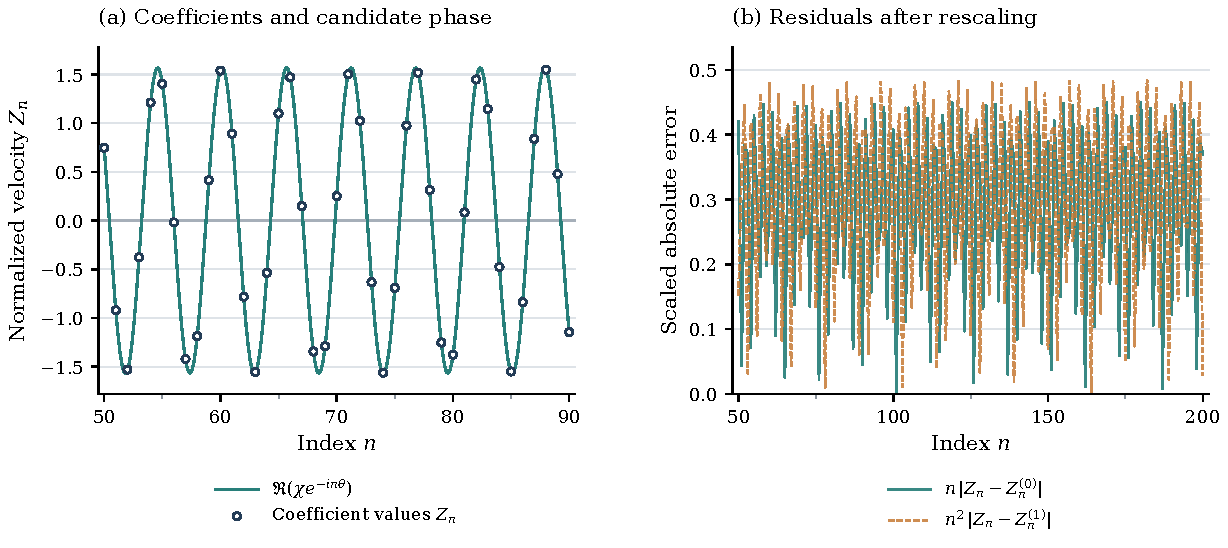
\includegraphics[width=\textwidth]{figures/diagonal_velocity_asymptotics.pdf}
\caption{Diagonal velocities and the proposed dominant conjugate pair.
Left: normalized coefficient values and the candidate oscillatory phase.
Right: leading and corrected normalized errors after multiplication
by $n$ and $n^2$. The coefficients have exact interval certificates;
the normalization and asymptotic comparison are numerical diagnostics
of Conjecture~\ref{diag:q:dominance}, not a proof of accessibility or dominance.}
\label{fig:diagonal-asymptotic}
\end{figure}

As a separate diagnostic of the local sign, the script follows the root
of \eqref{diag:q:inverse} numerically along $t=s t_*$, starting at
$u(0)=\log2$ and using successive warm Newton starts.  At the last tested
point, $1-s\approx3.76\,10^{-38}$, the estimate
$(u(s t_*)-u_*)/\sqrt{1-s}$ differs from $\chi$ by approximately
$1.8\,10^{-19}$, consistent with the next term of
\eqref{diag:q:puiseux}.  This computation was not initialized by imposing
the chosen local square-root sign.

These data support the proposed pair, local sign, and two coefficient
terms.  They do not certify continuation of a branch, prevent a numerical
root solver from changing sheets, or exclude an additional singularity of
smaller or equal modulus.  The main remaining analytic problem is to
prove or refute Conjecture~\ref{diag:q:dominance} on the inverse surface.
Even if it holds, questions about the density of positive velocities
require control of the rotation angle and of indices close to cosine
zeros; sign agreement on a finite range settles neither issue.

% Self-contained section for integration into the parent research article.
% Uses standard theorem/lemma/corollary/proposition environments and amsmath.
\section{The optimal exterior differential barrier}
\label{opt:sec:barrier}

The incoming report \emph{Lerch Global Phase} proves an exterior
one-crossing inequality with the fixed coefficient $e^{-n}$ and explicitly
asks for the optimum over all positive coefficients in its further-research
question~2. We solve that optimization problem. The sharp coefficient is
controlled by a cubic algebraic number; its large-index limit involves the
golden ratio. A distinction between a strict pointwise inequality and a
strict inequality for positive geometric sums is essential at the optimum.

For integers $n\geq2$ define
\begin{equation}\label{opt:eq:family}
 g_n(x)=\frac{(\log x)^{n-1}(n-\log x)}{x^2},\qquad
 U_n(a,\rho)=\sum_{m=0}^{\infty}\rho^m g_n(a+m).
\end{equation}
Here $a>0$ and $0\leq\rho\leq1$. The series and each fixed number
of its $a$ derivatives converge absolutely and locally uniformly,
uniformly in $\rho$, since the $m$th summand after $j$ derivatives is
$O(m^{-2-j}(1+\log^n m))$. For $\rho<1$, $U_n$ is the first
$a$ derivative of the order-$n$ Lerch coefficient
$\sum_{m\geq0}\rho^m\log^n(a+m)/(a+m)$; at $\rho=1$ it is
$\gamma_n'(a)$ in the usual Stieltjes Laurent convention.

Call a pair $(B,\lambda)$ \emph{uniformly admissible} if $B>0$,
$\lambda>0$, and
\begin{equation}\label{opt:eq:admissible}
 \partial_aU_n(a,\rho)+\lambda U_n(a,\rho)<0
 \qquad(a\geq B,\ 0<\rho\leq1).
\end{equation}
The uniformity down to arbitrarily small positive $\rho$ makes this a
precise optimization problem. A smaller cutoff at one fixed deformation
parameter is a different problem.

Put $\varphi=(1+\sqrt5)/2$. Let $r_n$ be the unique positive root of
\begin{equation}\label{opt:eq:cubic}
 r^3+nr^2-nr-n=0,
\end{equation}
and set
\begin{equation}\label{opt:eq:lambda}
 \tau_n=(2-r_n)e^{-r_n},\qquad \lambda_n=e^{-n}\tau_n,
 \qquad \Delta_n=\sqrt{n^2+8n},\qquad
 \alpha_n=\frac{3n-\Delta_n}{4}.
\end{equation}
For $0<\tau\leq1$, write
\begin{equation}\label{opt:eq:R}
 R_{n,\tau}(y)=2y^2-3ny+n(n-1)+\tau e^{y-n}y(n-y).
\end{equation}

\begin{theorem}[Optimal coefficient and optimal cutoff]
\label{opt:thm:optimal}
For every integer $n\geq2$ the following statements hold.
\begin{enumerate}
\item The cubic root satisfies $1<r_n<\varphi$. There is a unique
 $\eta_n\in(\alpha_n,(n-1)/2)$ such that
 $R_{n,\tau_n}(\eta_n)=0$. Put $B_n=e^{\eta_n}$.
\item The pointwise inequality is
 \begin{equation}\label{opt:eq:pointwise}
  g_n'(x)+\lambda_n g_n(x)\leq0\qquad(x\geq B_n).
 \end{equation}
 Equality occurs at exactly two points,
 \begin{equation}\label{opt:eq:equality-points}
  x=B_n\quad\hbox{and}\quad x=e^{n+r_n}.
 \end{equation}
\item The pair $(B_n,\lambda_n)$ is uniformly admissible. Every
 uniformly admissible pair $(B,\lambda)$ has $B\geq B_n$, and if
 $B=B_n$ then $\lambda=\lambda_n$.
\item Consequently $e^{\lambda_n a}U_n(a,\rho)$ is strictly decreasing
 on $[B_n,\infty)$ for every $0<\rho\leq1$. There is at most one
 zero there; any such zero is simple and crosses from positive to
 negative.
\end{enumerate}
\end{theorem}

We give a complete proof, including the boundary qualification.

\begin{lemma}[The negative-tail constraint]\label{opt:lem:tail}
For $r>0$ put
\[
 T_n(r)=2-\frac{n-1}{n+r}-\frac1r.
\]
The function $e^{-r}T_n(r)$ has a unique maximum, at $r=r_n$, and
\begin{equation}\label{opt:eq:Tmaximum}
 \max_{r>0}e^{-r}T_n(r)=(2-r_n)e^{-r_n}=\tau_n.
\end{equation}
Thus $\lambda_n$ is the smallest coefficient that can make
$g_n'+\lambda g_n\leq0$ on the whole interval $(e^n,\infty)$.
\end{lemma}
\begin{proof}
For $x=e^{n+r}>e^n$ one has $g_n(x)<0$ and
\[
 -\frac{g_n'(x)}{g_n(x)}=e^{-n-r}T_n(r).
\]
Dividing the desired inequality by the negative quantity $g_n(x)$
shows that it is equivalent to
$\lambda\geq e^{-n-r}T_n(r)$ for every $r>0$.

Now
\[
 T_n'(r)=\frac{n-1}{(n+r)^2}+\frac1{r^2}>0,
 \qquad
 T_n''(r)=-\frac{2(n-1)}{(n+r)^3}-\frac2{r^3}<0.
\]
Therefore $T_n'-T_n$ is strictly decreasing, tends to $+\infty$
at zero, and tends to $-2$ at infinity. It has precisely one zero,
which is the unique maximum of $e^{-r}T_n(r)$. The factorization
\begin{equation}\label{opt:eq:factor}
 (T_n-T_n')r^2(n+r)^2
 =(n+2r)(r^3+nr^2-nr-n)
\end{equation}
identifies that point with the positive root of \eqref{opt:eq:cubic}.
The cubic has exactly one positive root by its coefficient sign
variation, or by the preceding uniqueness argument. Its values at $1$
and $\varphi$ are $1-n<0$ and $\varphi^3>0$, respectively, giving
$1<r_n<\varphi$.

Rearranging the cubic gives
$n=r_n^3/(1+r_n-r_n^2)$. Substitution in $T_n(r_n)$ simplifies it
to $2-r_n$, proving \eqref{opt:eq:Tmaximum}. The maximum is positive;
the tail inequality is strict except at its unique maximizing point.
\end{proof}

\begin{lemma}[The positive-side cutoff]\label{opt:lem:cutoff}
For every $n\geq2$ and every $0<\tau\leq1$, the function
$R_{n,\tau}$ has exactly one root $\eta_n(\tau)$ in $(0,n)$.
It satisfies
\[
 \alpha_n<\eta_n(\tau)<\frac{n-1}{2},
 \qquad
 R_{n,\tau}(y)>0\ (0<y<\eta_n(\tau)),\qquad
 R_{n,\tau}(y)<0\ (\eta_n(\tau)<y\leq n).
\]
The root is simple, and $\eta_n(\tau)$ is strictly increasing in $\tau$.
\end{lemma}
\begin{proof}
For $y=n-t$, $0\leq t\leq(n+1)/2$, use
$\tau e^{-t}\leq(1+t)^{-1}$ and $(n-t)t\geq0$. This gives
\begin{align*}
 (1+t)R_{n,\tau}(n-t)
 &\leq2t^3+(1-n)t^2-nt-n\\
 &\leq2t^2-nt-n<0.
\end{align*}
For the second inequality use $2t\leq n+1$. The final quadratic is
convex, with negative values $-n$ and $(1-n)/2$ at the two endpoints,
so it is negative throughout. This proves negativity for
$(n-1)/2\leq y\leq n$.

On $0\leq y\leq(n-1)/2$,
\[
 R_{n,\tau}''(y)
 =4+\tau e^{y-n}\{-y^2+(n-4)y+2n-2\}>4.
\]
The bracket is a concave quadratic whose endpoint values are
$2(n-1)$ and $(n^2-1)/4$, both positive. Since $R_{n,\tau}(0)>0$
and $R_{n,\tau}((n-1)/2)<0$, strict convexity gives one and only one
crossing on this interval; a second crossing would force the function
to be nonnegative at its right endpoint. The derivative at the crossing
is strictly negative. The polynomial part vanishes at $\alpha_n$, so
$R_{n,\tau}(\alpha_n)>0$, proving the lower bound. Finally
\[
 \frac{\partial\eta_n(\tau)}{\partial\tau}
 =-\frac{e^{\eta_n(\tau)-n}\eta_n(\tau)(n-\eta_n(\tau))}
 {\partial_yR_{n,\tau}(\eta_n(\tau))}>0.
\]
\end{proof}

\begin{proof}[Proof of Theorem~\ref{opt:thm:optimal}]
For $x=e^y>1$, differentiation gives
\begin{equation}\label{opt:eq:pointwise-factor}
 g_n'(x)+\tau e^{-n}g_n(x)
 =x^{-3}y^{n-2}R_{n,\tau}(y).
\end{equation}
The prefactor is positive. Because $1<r_n<\varphi<2$,
$0<\tau_n<1$. Lemma~\ref{opt:lem:cutoff} treats the region below
$e^n$, Lemma~\ref{opt:lem:tail} treats the region above it, and
at $x=e^n$ one has $g_n'<0$. This proves the nonpositive inequality
and the exact equality set.

For $a\geq B_n$, every summand in
\[
 (\partial_a+\lambda_n)U_n(a,\rho)
 =\sum_{m=0}^{\infty}\rho^m
       [g_n'(a+m)+\lambda_n g_n(a+m)]
\]
is nonpositive. Only two possible arguments can give equality.
When $\rho>0$, at least one of the three summands $m=0,1,2$ is
strictly negative, so the sum is strictly negative. Absolute convergence
justifies the differentiation and summation, also at $\rho=1$.

To prove optimality, suppose first that $\lambda<\lambda_n$.
At $x_*=e^{n+r_n}$, where $g_n(x_*)<0$, one has
$g_n'(x_*)+\lambda g_n(x_*)>0$. Since
$(\partial_a+\lambda)U_n(a,\rho)$ tends to this pointwise expression
as $\rho\downarrow0$, every cutoff $B\leq x_*$ fails for small
positive $\rho$. In particular, such a coefficient cannot beat $B_n$.
If $\lambda\geq\lambda_n$ and $B<B_n$, choose
$\max(B,1)<a<B_n$. Then $g_n(a)>0$ and
\[
 g_n'(a)+\lambda g_n(a)
 \geq g_n'(a)+\lambda_n g_n(a)>0,
\]
again contradicting admissibility at sufficiently small positive $\rho$.
This proves $B\geq B_n$. At $B=B_n$, any $\lambda>\lambda_n$
makes the pointwise expression strictly positive at $a=B_n$,
so only $\lambda_n$ is possible. The integrating factor and the sign
of the derivative at any zero prove the last assertion.
\end{proof}

\paragraph{Why the pointwise strict optimum is not attained.}
If the requirement is instead
$g_n'(x)+\lambda g_n(x)<0$ for every $x>B$, the infimum of possible
cutoffs is still $B_n$, but no coefficient attains it. At
$\lambda_n$ the outer point $e^{n+r_n}>B_n$ has equality.
Coefficients $\lambda>\lambda_n$, sufficiently close to $\lambda_n$,
have strict tail inequality and cutoff $e^{\eta_n(e^n\lambda)}$
decreasing to $B_n$ as $\lambda\downarrow\lambda_n$.
The strict summed theorem therefore must not be copied verbatim into
a statement about every positive measure or about the elementary
endpoint $\rho=0$.

\paragraph{Positive measures.}
Let $\nu$ be a nonzero positive measure on $[0,\infty)$ satisfying
\[
 \int_{[0,\infty)}\frac{1+\log^n(2+t)}{(1+t)^2}\,d\nu(t)<\infty.
\]
This condition supplies locally uniform domination of the integral
and its derivative. The function
$H_n(a)=\int g_n(a+t)\,d\nu(t)$ satisfies
$H_n'+\lambda_nH_n\leq0$ for $a\geq B_n$. It is strictly negative
unless the measure is supported on the at most two points for which
$a+t$ belongs to \eqref{opt:eq:equality-points}. In particular,
non-atomic measures and measures with at least three support points
give the strict inequality. This is the exact measure-theoretic
qualification forced by the optimal tangency.

\subsection{The golden-ratio limit and convergent coefficient formulas}
\label{opt:sec:asymptotic}

\begin{theorem}[Monotone optimizer and its large-index expansion]
\label{opt:thm:asymptotic}
The sequence $r_n$ strictly increases to $\varphi$, whereas
$\tau_n=e^n\lambda_n$ strictly decreases to
$\tau_\infty=(2-\varphi)e^{-\varphi}$. As $n\to\infty$,
\begin{align}
 r_n={}&\varphi-
 \left(1+\frac{2\sqrt5}{5}\right)\frac1n
 +\left(\frac52+\frac{57\sqrt5}{50}\right)\frac1{n^2}
 +O(n^{-3}),\label{opt:eq:r-asymptotic}\\
 \lambda_n={}&e^{-n}\tau_\infty
 \left[1+\frac{7+3\sqrt5}{2n}
 -\frac{35+16\sqrt5}{10n^2}+O(n^{-3})\right].
 \label{opt:eq:lambda-asymptotic}
\end{align}
Writing $\epsilon=1/n$, the complete expansion of $r_n$ is a
convergent power series for $|\epsilon|<5/27$. Its coefficients are
\begin{equation}\label{opt:eq:r-Lagrange}
 r(\epsilon)=\varphi+
 \sum_{j\geq1}\frac{(-\epsilon)^j}{j}
 [z^{j-1}]
 \left(\frac{(\varphi+z)^3}{\sqrt5+z}\right)^j.
\end{equation}
In particular this is a convergent formula for every integer $n\geq6$.
\end{theorem}
\begin{proof}
The identity
$n=r^3/(1+r-r^2)$ has strictly positive derivative on $1<r<\varphi$:
\[
 \frac{d}{dr}\frac{r^3}{1+r-r^2}
 =\frac{r^2(3+2r-r^2)}{(1+r-r^2)^2}>0.
\]
It tends to infinity at $\varphi$, proving the claims about $r_n$.
Since $d[(2-r)e^{-r}]/dr=(r-3)e^{-r}<0$ in this interval,
the claims about $\tau_n$ follow.

The implicit equation
$\epsilon r^3+r^2-r-1=0$ has derivative $\sqrt5$ in $r$ at
$(\epsilon,r)=(0,\varphi)$, so the analytic implicit-function theorem
applies. Substitution of a quadratic series gives
\eqref{opt:eq:r-asymptotic}, and substitution into $(2-r)e^{-r}$ gives
\eqref{opt:eq:lambda-asymptotic}. With $r=\varphi+z$ the equation becomes
\[
 z=-\epsilon\frac{(\varphi+z)^3}{\sqrt5+z}.
\]
Lagrange inversion gives \eqref{opt:eq:r-Lagrange}.

For completeness the convergence radius can be identified exactly.
The discriminant in $r$ is
\[
 \operatorname{disc}_r(\epsilon r^3+r^2-r-1)
 =(1-\epsilon)(27\epsilon+5).
\]
The branch selected at zero is holomorphic throughout
$|\epsilon|<5/27$: away from zero the discriminant is nonzero there,
and the selected branch has a removable, already analytic continuation
at zero. Along the real interval $-5/27<\epsilon\leq0$ this branch
increases from $\varphi$ to $3$. At $(\epsilon,r)=(-5/27,3)$,
the first $r$ derivative vanishes while
$\partial_\epsilon=27$ and $\partial_r^2=-4/3$ are nonzero.
It is therefore a genuine square-root branch point. Hence the Taylor
radius is exactly $5/27$.
\end{proof}

\subsection{The exponentially small displacement of the cutoff}
The optimizer has an ordinary convergent expansion in $1/n$. The
cutoff also contains an exponentially small displacement in logarithmic
coordinates, which should be kept separate from that algebraic expansion.
Put
\[
 E_n=e^{\alpha_n-n},\qquad A_n=\alpha_n(n-\alpha_n),
 \qquad C_n=n-2\alpha_n.
\]

\begin{theorem}[Cutoff expansion and an all-orders formula]
\label{opt:thm:cutoff-expansion}
As $n\to\infty$,
\begin{align}
 \eta_n={}&\alpha_n+
 \frac{\tau_nA_n}{\Delta_n}E_n\notag\\
 &+\tau_n^2\left[
 \frac{A_n(A_n+C_n)}{\Delta_n^2}
 +\frac{2A_n^2}{\Delta_n^3}\right]E_n^2
 +O(n^3E_n^3).\label{opt:eq:eta-two-sectors}
\end{align}
Every further power of $E_n$ has an explicit coefficient. More precisely,
for all sufficiently large $n$ the solution $\delta=\eta_n-\alpha_n$
is obtained, at $E=E_n$, from the locally convergent series
\begin{equation}\label{opt:eq:eta-Lagrange}
 \delta(E)=\sum_{j\geq1}\frac{E^j}{j}[z^{j-1}]
 \left[
 \frac{\tau_ne^z(\alpha_n+z)(n-\alpha_n-z)}{\Delta_n-2z}
 \right]^j.
\end{equation}
For each fixed truncation order $J$, its error at $E_n$ is
$O_J(n^{J+1}E_n^{J+1})$.
In the original $a$ coordinate this implies
\begin{equation}\label{opt:eq:B-asymptotic}
 B_n=e^{\alpha_n}+
 \frac{\tau_\infty}{4e^2}
 \left(n+\frac{7+3\sqrt5}{2}\right)+O(n^{-1}).
\end{equation}
The leading additive displacement above the first stationary point
of $g_n$ has coefficient
\[
 \frac{\tau_\infty}{4e^2}=0.0025625510827\ldots.
\]
\end{theorem}
\begin{proof}
Substitute $\eta_n=\alpha_n+\delta$ in its defining equation and use
the exact quadratic Taylor expansion of the polynomial part:
\[
 -\Delta_n\delta+2\delta^2+
 \tau_n E_ne^\delta(\alpha_n+\delta)(n-\alpha_n-\delta)=0.
\]
Equivalently, $\delta=E_nf_n(\delta)$ with
\[
 f_n(z)=
 \frac{\tau_ne^z(\alpha_n+z)(n-\alpha_n-z)}{\Delta_n-2z}.
\]
This proves \eqref{opt:eq:eta-Lagrange} by Lagrange inversion. Its
first two coefficients are $f_n(0)$ and $f_n(0)f_n'(0)$, giving
\eqref{opt:eq:eta-two-sectors}.

The remainder statement can be justified uniformly in $n$. On a fixed
small complex disk in $z$, $f_n$ and its derivative are $O(n)$, while
$\Delta_n\asymp n$. For $|E|<c/n$ with a sufficiently small absolute
$c>0$, the map $z\mapsto Ef_n(z)$ is a contraction of a smaller
fixed disk. The analytic solution is uniformly bounded there. Cauchy
estimates therefore bound its $j$th coefficient by $O(C^jn^j)$.
Since $E_n\asymp e^{-n/2}$, every fixed-order tail has the asserted
bound for sufficiently large $n$.

Finally exponentiate the first sector. Its omitted terms become
$O(n^2e^{-n/2})$ after multiplication by $e^{\alpha_n}$. Direct
expansion gives
\[
 \frac{A_n}{\Delta_n}e^{2\alpha_n-n}
 =e^{-2}\left(\frac n4-\frac1n+O(n^{-2})\right).
\]
Combining this with \eqref{opt:eq:lambda-asymptotic} yields
\eqref{opt:eq:B-asymptotic}. No relative approximation to
$\eta_n-\alpha_n$ is being inferred from an uncontrolled algebraic
remainder in $\alpha_n$.
\end{proof}

\paragraph{Limits of the conclusion.}
The optimum is over constant first-order operators, required uniformly
for all positive geometric weights down to $\rho=0$. It does not
optimize variable-coefficient operators, inequalities only at the zeros,
or cutoffs at one fixed $\rho$. Those extensions remain separate
research questions. In particular, improving an exterior barrier does
not on its own classify all interior zeros or prove a global
monotonicity theorem for individual zero branches.

\section{Reproducible computations and numerical illustrations}
\label{sec:computations}

\subsection{What the checks establish}

The package separates three different forms of evidence.
The general theorems are proved in the preceding sections.
Exact finite checks verify rational identities or enclose particular
numbers using a proved remainder bound. Floating-point computations
check conventions and illustrate asymptotic behavior. The last category
is not used to certify equality, a zero count, or a decimal enclosure.

The harmonic verifier uses two independent exact constructions through
order thirty. One differentiates the kernel in the form
\[
 K^{(j)}(t)=
 \frac{\sqrt y}{(1+y)^{j+1}}
 \{P_j(y)\log(1+y)+Q_j(y)\},\qquad y=e^{-2t}.
\]
The other constructs $\sec z$ and
$\sec z\log\sec z$ by rational formal power-series operations.
The resulting rational and $\log2$ coefficients agree at all thirty-one
nonpositive integer arguments. The same program checks the polynomial
in the proof of $K''>0$, the rational constant $181/27$, and the
right-half-plane tail bound.

The diagonal verifier compares the Stirling expression with the
independently derived quadratic recurrence in $\mathbb Q[L]$
through $n=40$. It also checks the inverse generating equation
through degree forty after a rational formal specialization.
A positive-series enclosure of $\log2$, followed by rational interval
Horner evaluation, certifies the velocity signs for $2\le n\le40$.
The separate quantitative experiment extends exact sign enclosures
to $50\le n\le200$ and compares them with the conjectured singularity
asymptotic. Its analytic continuation and asymptotic comparisons remain
numerical diagnostics.

The barrier verifier checks ten exact symbolic identities, including
the critical-point factorization, the cubic discriminant, and the displayed
inverse-index coefficients. For $n=2,3,4,5,10,25,100$ it also isolates
the optimizer and cutoff by exact rational interval arithmetic.
The exponential evaluator reduces its argument to $[0,1]$,
uses a Taylor polynomial with the explicit tail bound
$2/(M+1)!$, and then applies outward-rounded inversion and repeated
squaring. Thus the recorded decimal endpoints are consequences of
rational comparisons, rather than the output of a floating-point
root finder.

\subsection{Harmonic zeros and the two asymptotic scales}

Table~\ref{tab:harmonic-zeros} lists diagnostic roots from the positive
Mellin-moment ratio. The first three were also substituted into
independent differentiated-kernel Mellin integrals.
Those checks do not share the digamma representation.
At forty-five working decimal digits, the three independent absolute
residuals are approximately $2.1\times10^{-43}$,
$1.1\times10^{-31}$, and $1.2\times10^{-25}$.
Working precision is not a guarantee of correct output digits, and
these values are not presented as certified intervals.

\begin{table}[htbp]
\centering
\begin{tabular}{@{}r r r@{}}
\toprule
$m$ & Approximate $\sigma_m$ & Approximate $\varepsilon_m$\\
\midrule
1   & $-2.151826895870$    & $0.848173104130$\\
2   & $-4.358674064874$    & $0.641325935126$\\
3   & $-6.454482934804$    & $0.545517065196$\\
5   & $-10.548589016994$   & $0.451410983006$\\
10  & $-20.640881124485$   & $0.359118875515$\\
50  & $-100.764467222239$  & $0.235532777761$\\
500 & $-1000.845421933140$ & $0.154578066860$\\
\bottomrule
\end{tabular}
\caption{Numerical illustrations of the proved real-zero classification.
The decimals are diagnostic approximations.}
\label{tab:harmonic-zeros}
\end{table}

\begin{figure}[htbp]
\centering
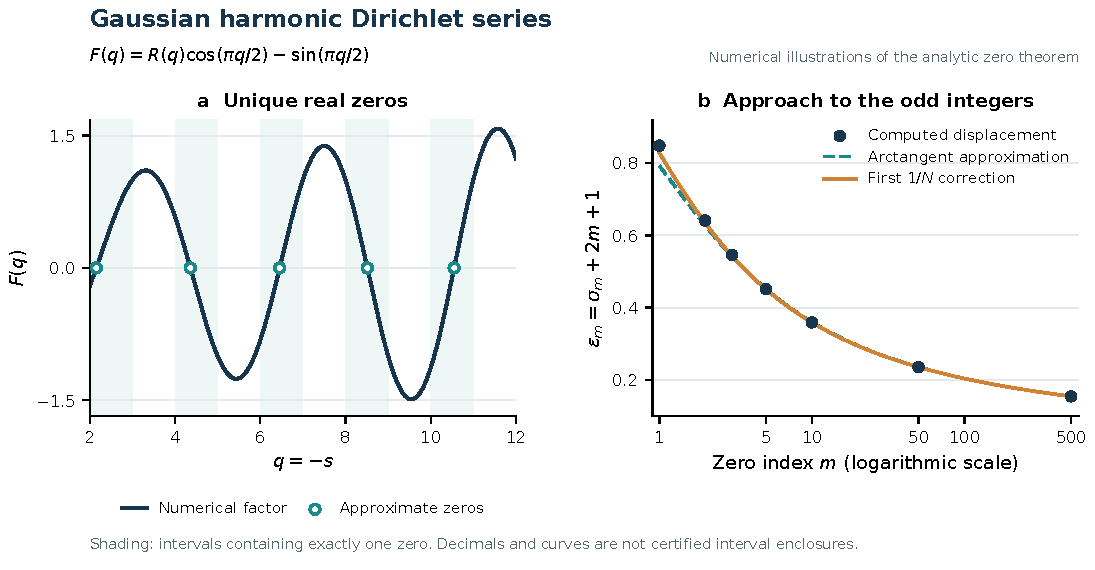
\includegraphics[width=\textwidth]{figures/harmonic_order_zeros.pdf}
\caption{The normalized Fourier factor and the real-zero displacement.
Zeros of $R(q)\cos(\pi q/2)-\sin(\pi q/2)$ give the real zeros of
$S(-q)$ because its omitted prefactor is positive.
The displacement plot compares numerical roots with the arctangent
term and its first $1/N$ correction. These curves illustrate
Theorems~\ref{sorder:thm:all-real-zeros}
and \ref{sorder:thm:zero-asymptotic}; they are not their proofs.}
\label{fig:harmonic}
\end{figure}

The first inverse-index correction need not improve an approximation
at every small index. For example, at $m=5$ the leading arctangent
term happens to be unusually close, and its next term overshoots.
The theorem concerns controlled errors as $m\to\infty$ and does not
assert a globally enveloping expansion. The distinction between the
inverse-logarithmic series and the smaller $1/N$ sectors is also
essential: retaining more logarithmic powers alone cannot resolve
an algebraically small correction in $N$.

\subsection{Certified sample cutoffs}

The cutoff enclosures in Table~\ref{tab:cutoffs} are exact.
The old fixed-coefficient cutoffs in its last column are rounded
diagnostics for comparison. In particular, the new coefficient can
reduce the compact interval remaining for a separate zero count.
That improvement does not itself supply signs on the compact interval.

\begin{table}[htbp]
\centering
\small
\begin{tabular}{@{}r l r@{}}
\toprule
$n$ & Certified enclosure for $B_n$ &
Fixed $\lambda=e^{-n}$ cutoff\\
\midrule
2 & $[1.47580064163065338930,\;1.47580064163065338931]$
  & $1.5102804080$\\
3 & $[2.27333271490894820528,\;2.27333271490894820529]$
  & $2.3431706385$\\
4 & $[3.57479611518613398335,\;3.57479611518613398336]$
  & $3.6783274602$\\
5 & $[5.69074542139040729581,\;5.69074542139040729582]$
  & $5.8264887639$\\
10 & $[63.21469931898564283555,\;63.21469931898564283556]$
  & $63.5050628049$\\
\bottomrule
\end{tabular}
\caption{Exact sample enclosures for the least uniform cutoff.
Full optimizer, coefficient, and logarithmic-cutoff intervals are
recorded in the accompanying JSON certificate.}
\label{tab:cutoffs}
\end{table}

\begin{figure}[htbp]
\centering
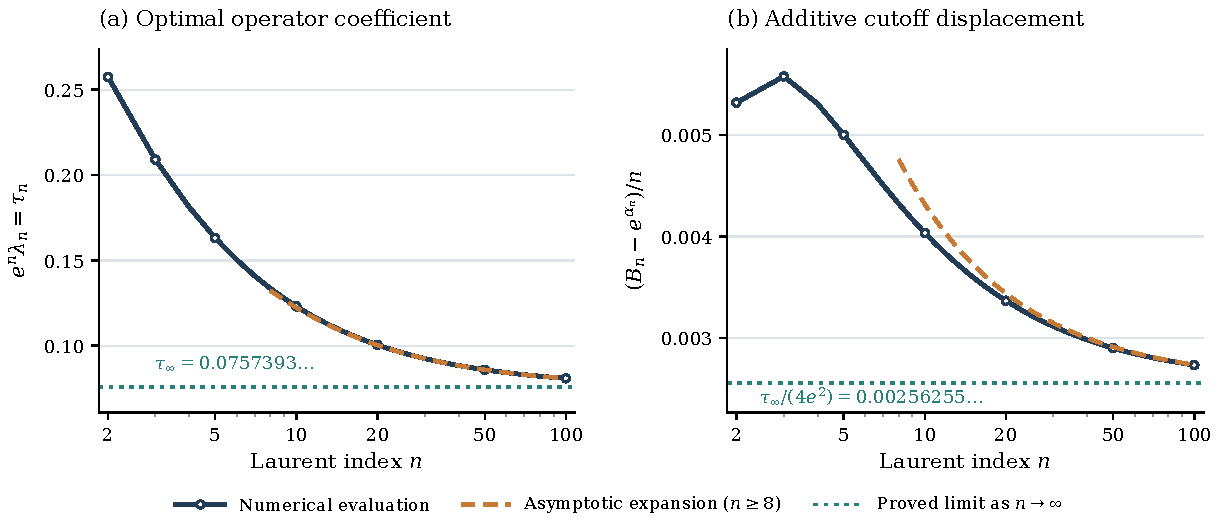
\includegraphics[width=\textwidth]{figures/optimal_barrier_parameters.pdf}
\caption{Optimal exterior-barrier parameters. Navy curves show numerical
evaluations of the proved defining formulas; teal dotted lines show
the limiting constants. Orange dashed curves, displayed for $n\ge8$,
use two inverse-index corrections for $\tau_n$ and the first correction
for the normalized cutoff displacement. Numerical evaluation illustrates
the analytic theorems; exact sample enclosures are recorded separately.}
\label{fig:barrier}
\end{figure}

For the figure, the difference $B_n-e^{\alpha_n}$ is evaluated as
$e^{\alpha_n}\operatorname{expm1}(\eta_n-\alpha_n)$ at high precision.
Subtracting the two large exponentials directly would obscure the
small displacement and can produce a misleading numerical comparison.

\subsection{Replay and build instructions}

The archive contains the complete expanded \nolinkurl{article.tex},
the modular section sources, the compiled PDF, the data records,
and all verification and plotting scripts.
The standard-library exact checks and the symbolic/interval checks
have separate entry points:
\begin{minipage}{\textwidth}
\begin{verbatim}
python3 code/verify_diagonal.py
python3 code/verify_gaussian_order.py --output data/gaussian_exact.json
python3 code/verify_optimal_barrier.py \
  --output data/optimal_barrier_verification.json
\end{verbatim}
\end{minipage}
The full numerical and quantitative commands, package requirements,
and figure regeneration steps are in \nolinkurl{README.md}.
The optional numerical routines use mpmath, and the scientific figures
use Matplotlib and SciPy. A requirements file records the environment
used for the delivered run.

To regenerate the expanded TeX and PDF from the modular sources:
\begin{verbatim}
python3 code/assemble_article.py
latexmk -pdf -interaction=nonstopmode -halt-on-error article.tex
\end{verbatim}
The distributed PDF was built from the same expanded source and
visually checked. The build and verification records are included.
The source snapshot identifies the baseline for later integration;
the package does not modify the remote repository.

\section{Manuscript corrections and integration}
\label{sec:corrections}

\subsection{Replace the broad monotonicity suggestion by a quantified question}

The final research chapter still says that monotonicity of higher zero
branches in the deformation parameter is suggested by the first
correction \cite{ProjectDiscovery}. Read literally as a direction for
all indices, that suggestion is obsolete once the incoming results are
taken into account. The earlier boundary and bifurcation reports already
give a turning lower branch at $(n,k)=(2,1)$, while the global-phase
report proves an increasing middle branch at $(3,1)$
\cite{IncomingBoundary,IncomingBifurcation,IncomingPhase}.
The positive initial velocity at $(n,k)=(4,3)$ also appears in the
formal-reductions report \cite{IncomingReductions}.

The additional correction supplied here is infinite in scope:
Theorem~\ref{diag:thm:oscillation} gives both directions at arbitrarily
large indices on $k=n-1$. A replacement paragraph should therefore
ask for \emph{effective derivative-order thresholds depending on the
Laurent index}, the distribution of turning points below those
thresholds, and the joint-index scales on which a uniform direction
does emerge. It should not suggest that every higher branch decreases
throughout the deformation.

One precise consequence is Corollary~\ref{diag:cor:threshold}:
if $K_n$ guarantees decreasing motion for every branch and every
$k\ge K_n$, then $K_n>n-1$ for infinitely many $n$.
This does not disprove the existence of $K_n$, does not show that
$K_n/n$ is unbounded, and does not identify a saturation threshold
for the number of zeros. Those are different claims.

\subsection{Record the exact endpoint in the optimized barrier}

The solution of the incoming exterior-operator problem should be recorded
in two parts. The least uniform cutoff for the summed family is attained
and its inequality is strict when $\rho>0$. The strict pointwise cutoff
has the same infimum, but the infimum is not attained. At the optimal
coefficient,
\[
 g_n'(x)+\lambda_ng_n(x)=0
 \quad\Longleftrightarrow\quad
 x\in\{B_n,e^{n+r_n}\},\qquad x\ge B_n.
\]
Consequently the strict summed theorem must not be extended unchanged to
$\rho=0$, to arbitrary one- or two-point positive measures, or to a
claim that every individual summand is strictly negative.
Theorem~\ref{opt:thm:optimal} and its positive-measure extension state
the exact hypotheses. This is a qualification of the newly optimized
result, not an assertion that the earlier fixed-coefficient theorem
was false.

\subsection{Keep integer special values separate from order-zero geometry}

For reference, write
$g_{a,b}=\operatorname{Im}\operatorname{Li}_{a,b}(i,1)$ and
$G=\beta(2)$. The remaining manuscript conjecture is
\begin{align}
 S(6)\stackrel{?}{={}}&
 \frac{722}{527}g_{6,1}+\frac{40}{527}g_{4,3}
 -\frac{128}{155}g_{2,5}+\frac{15191}{28569600}\pi^7
 \notag\\
 &-\frac3{124}G\zeta(5)
 -\frac{2373}{10540}\beta(4)\zeta(3)
 -2\beta(6)\log2 .
 \label{eq:retained-S6}
\end{align}
This is quoted to identify the open target, not proposed as a new
identity. The exact shuffle relation already in the manuscript is
\begin{align}
 g_{2,5}={}&30g_{6,1}+15g_{5,2}+5g_{4,3}
 -\frac{15}{512}G\zeta(5)\notag\\
 &+\frac3{16}\beta(4)\zeta(3)-\frac{11\pi^7}{368640}.
 \label{eq:retained-basket-change}
\end{align}
It proves equivalence of the two reported $S_6$ baskets
\cite{ProjectQuotients}. It does not prove their residual vanishes.

Our Fourier--beta identity gives new exact representations of $S(6)$
by analytic continuation, but does not reduce it to the specified
weight-seven period basket. Entirety and a complete real zero set
likewise do not imply that reduction. The finite separating functional
in the manuscript obstructs a particular restricted
shuffle/stuffle presentation; it does not prove arithmetic independence.
The successful $S_4$ certificate shows why a convergent octahedral
relation and suitable higher-depth lifts are natural next ingredients
\cite{ProjectS4,ProjectQuotients}.

The incoming rejected $S_8$ vector is a useful methodological boundary:
an interval containing zero is compatible with equality, but does not
prove it; a certified interval excluding zero rejects the specific
frozen vector, but does not prove independence of its basket.
The proposed integration preserves those distinctions
\cite{ProjectDiscovery}.

\subsection{Notation and reusable proof components}

The generalized secant numbers in
Corollary~\ref{sorder:cor:negative-values} are positive at $\alpha=1$.
They differ by $(-1)^m$ from the signed Euler numbers sometimes defined
through $\sech t$. Their generating function, not the letter $E$ alone,
fixes the convention.
The symbols $S_p$ and $S(p)$ agree at positive integers. At negative
integers $S(s)$ always denotes analytic continuation, since the
original alternating Dirichlet series no longer converges.

The harmonic continuation and its Fourier identity can be integrated
after the Gaussian harmonic sums. The diagonal theorem belongs after
the elementary endpoint and fixed-index Lerch zero geometry. The
optimized barrier should follow the incoming global-phase theorem,
with its research question~2 marked resolved with the attainment
qualification above. A suggested replacement paragraph and dependency
map are included in the integration artifacts.

\section{A proposed research programme}
\label{sec:programme}

The results suggest several specific next problems. Each item below
states what is missing and what would count as progress.

\subsection{The order interpolation and its zeros}

\paragraph{1. Nonreal zeros and growth of the entire function.}
Determine the growth order and directional indicator of $S(s)$, then
locate and count its nonreal zeros. The real classification and the
zero-free half-plane $\Re s\ge3$ are starting constraints, not a
classification in the complex plane. A useful first target is a rigorous
argument-principle count in bounded rectangles using regularized Mellin
integrals and controlled tails. A global conclusion would require
uniform complex asymptotics.

\paragraph{2. Explicit finite-index errors for $\sigma_m$.}
Replace the implicit constants in
Theorem~\ref{sorder:thm:zero-asymptotic} by computable bounds valid for
every $m$ beyond a stated threshold. The proof already reduces this
to a sectorial digamma remainder and beta-series estimates.
Combining those with a lower bound on the derivative of the tangent
comparison would give certified intervals of predictable width
without numerical root scanning.

\paragraph{3. Shifted denominators and higher harmonic depth.}
Study
\[
 S_a(s)=\sum_{n\ge0}\frac{(-1)^nH_n}{(n+a)^s},
 \qquad a>0,
\]
and the elementary-symmetric harmonic sums already used by the
manuscript. Their Mellin kernels are explicit, but the self-reflecting
choice $a=1/2$ is special: its Fourier transform gives the positive
moment ratio used here. Determine which shifts preserve a comparable
sign or total-positivity structure. It would be premature to assert
the same real zero pattern for every shift.

\paragraph{4. Sharper moment-ratio inequalities.}
The estimate $R'(q)<\sqrt{181/27}/q$ is intentionally coarse.
Find the best constant or a useful pointwise comparison, and determine
whether $R'$ decreases on $[2,\infty)$. The proof establishes neither
concavity nor complete monotonicity of $R$. A refined covariance
inequality may be more efficient than additional moment bounds.

\subsection{Joint-index Lerch geometry}

\paragraph{5. Prove or refute the accessible-singularity conjecture.}
The exact inverse equation for $u_A$ makes its finite critical values
explicit, but those values belong to different analytic sheets.
For $A=2$, prove which critical points are accessible from the germ
at zero, identify all singularities on its convergence circle, and
establish the continuation domain needed for coefficient transfer.
This would turn the quantitative conjecture into an asymptotic theorem.
Numerical radial continuation and agreement of many coefficients
are evidence, not a substitute for that domain argument.

\paragraph{6. Density and gaps of the two velocity signs.}
Theorem~\ref{diag:thm:oscillation} proves infinitude of both signs without
a density or a maximum gap. A dominant-conjugate-pair theorem should
give an oscillatory law, but a density statement also depends on the
arithmetic and possible resonances of its phase. For algebraic
$A>1$, the finite Stirling formula already excludes a zero velocity;
it does not bound how small a nonzero velocity may be.

\paragraph{7. Effective monotonicity thresholds.}
Determine the growth of the least $K_n$ for which all zero branches
decrease for $k\ge K_n$. The present lower constraint
$K_n>n-1$ along infinitely many indices should be combined with the
existing fixed-$n$ concentration estimates. A linear upper bound,
a sharp transition ratio, or a proof that no linear bound is possible
would each be meaningful outcomes; none follows merely from the
diagonal sign theorem.

\paragraph{8. Central root splitting for $n=k+r$.}
For fixed $r>1$, the elementary root at $a=1$ has multiplicity $r$.
Its natural perturbation can involve fractional powers of $\rho$.
Derive a uniform local normal form, determine the number of real
branches it produces, and compare it with the existing expansions
near positive Bessel zeros \cite{IncomingBessel}. The central root
and positive Bessel roots should not be treated as interchangeable
regimes.

\paragraph{9. Beyond first-order velocity.}
Find generating functions for higher $\rho$ derivatives of
$a_n^{(h)}(\rho)$ and for the size of the neighborhood in which
the first derivative determines its motion. Small nonzero
$v_n$ can force second-order terms to become relevant unusually early.
This is a concrete way to connect the local oscillation theorem
to actual turning points in the full deformation.

\subsection{Exterior barriers and remaining phase questions}

\paragraph{10. Fixed-parameter and variable-coefficient barriers.}
Theorem~\ref{opt:thm:optimal} optimizes a constant coefficient uniformly
for arbitrarily small positive $\rho$. For a fixed positive $\rho$, the tail sum may allow
a smaller cutoff. Determine the optimum as a function of $\rho$,
or allow a controlled positive function $\lambda(a)$.
Such an extension must specify its admissible class; otherwise a
best-operator question is not a well-defined optimization problem.

\paragraph{11. Existence inside the exterior uniqueness region.}
The optimal barrier proves at most one exterior zero and a downward
crossing. It does not guarantee a zero. Prove signs at $B_n$ for useful
ranges of $(n,\rho)$, perhaps using a small set of exact separators
and geometric-weight inequalities. This would turn a one-crossing
bound into an all-index existence and uniqueness theorem.

\paragraph{12. Strict span unimodality at index three.}
The incoming report already proves the exact unit maximum and its
nondegeneracy, but its stronger conjecture of strict increase before
the maximum and strict decrease afterwards remains open
\cite{IncomingPhase}. Additional control of the averaged outer slope
is required; the sign of the shifted-root identity alone does not
settle this shape question.

\subsection{Arithmetic reductions and formal verification}

\paragraph{13. A weight-seven mixed certificate.}
For \eqref{eq:retained-S6}, seek a convergent octahedral relation whose
image is nonzero under the known restricted separating functional.
Then lift and eliminate depth-three or higher terms with exact rational
rows. The useful output is a short certificate with an independently
specified word convention and regularization, rather than another
decimal relation fit. A failed search in a finite row space should be
recorded as a limitation of that row space.

\paragraph{14. Formalize the finite and analytic interfaces separately.}
The Stirling-polynomial recurrence, cubic factorization, rational
interval operations, and negative-integer recurrences are finite
targets suited to proof-assistant formalization. The subsequent
analytic targets are Mellin subtraction, the one-dimensional variance
inequality, the positive-coefficient argument, and the implicit
zero comparison. The current package provides ordinary proofs and
executable checks; it does not claim a completed Lean or other
proof-assistant verification.

\begin{thebibliography}{99}
\raggedright
\addcontentsline{toc}{section}{References}

\bibitem{Project}
V. Reshetnikov, \emph{ProveIt: Polylogarithm manuscript and incoming research},
repository snapshot at commit
\texttt{a0a90ef31877f98be437191c48b46f02d5456867},
10 October 2026.
\href{https://github.com/VladimirReshetnikov/ProveIt/tree/a0a90ef31877f98be437191c48b46f02d5456867/Analysis/Polylogarithms/docs/manuscript}{Pinned manuscript};
\href{https://github.com/VladimirReshetnikov/ProveIt/tree/a0a90ef31877f98be437191c48b46f02d5456867/docs/incoming}{pinned incoming directory}.

\bibitem{ProjectS4}
\emph{The mixed Gaussian weight-five identity and its exact proof},
chapter source \nolinkurl{04-S4-proof.tex}, in \cite{Project}.
\href{https://github.com/VladimirReshetnikov/ProveIt/blob/a0a90ef31877f98be437191c48b46f02d5456867/Analysis/Polylogarithms/docs/manuscript/chapters/04-S4-proof.tex}{Pinned source}.

\bibitem{ProjectQuotients}
\emph{Cyclotomic quotients and the weight-seven mixed candidate},
chapter source \nolinkurl{04-cyclotomic-quotients.tex}, particularly
the two-basket proposition and the $S_6$ conjecture, in \cite{Project}.
\href{https://github.com/VladimirReshetnikov/ProveIt/blob/a0a90ef31877f98be437191c48b46f02d5456867/Analysis/Polylogarithms/docs/manuscript/chapters/04-cyclotomic-quotients.tex}{Pinned source}.

\bibitem{ProjectGeometry}
\emph{Stieltjes--Lerch zero geometry},
chapter source \nolinkurl{09-zero-geometry.tex}, in \cite{Project}.
\href{https://github.com/VladimirReshetnikov/ProveIt/blob/a0a90ef31877f98be437191c48b46f02d5456867/Analysis/Polylogarithms/docs/manuscript/chapters/09-zero-geometry.tex}{Pinned source}.

\bibitem{ProjectDiscovery}
\emph{Research questions and discovery},
chapter source \nolinkurl{10-discovery.tex}, particularly the
higher-branch monotonicity direction and the frozen $S_8$ exclusion,
in \cite{Project}.
\href{https://github.com/VladimirReshetnikov/ProveIt/blob/a0a90ef31877f98be437191c48b46f02d5456867/Analysis/Polylogarithms/docs/manuscript/chapters/10-discovery.tex}{Pinned source}.

\bibitem{IncomingBoundary}
\emph{Lerch boundary research},
incoming archive \nolinkurl{proveit_lerch_boundary_research.zip},
source \nolinkurl{polylog_lerch_boundary/article.tex}, in \cite{Project}.
\href{https://github.com/VladimirReshetnikov/ProveIt/blob/a0a90ef31877f98be437191c48b46f02d5456867/docs/incoming/proveit_lerch_boundary_research.zip}{Pinned archive}.

\bibitem{IncomingBifurcation}
\emph{Lerch zero bifurcations},
incoming archive \nolinkurl{proveit_lerch_zero_bifurcations.zip},
source \nolinkurl{article/lerch_zero_bifurcations.tex}, in \cite{Project}.
\href{https://github.com/VladimirReshetnikov/ProveIt/blob/a0a90ef31877f98be437191c48b46f02d5456867/docs/incoming/proveit_lerch_zero_bifurcations.zip}{Pinned archive}.

\bibitem{IncomingPhase}
\emph{Lerch Global Phase},
incoming archive \nolinkurl{ProveIt_Lerch_Global_Phase_2026-10-09.zip},
source \nolinkurl{article/lerch_global_phase.tex},
especially further-research questions 1 and 2, in \cite{Project}.
\href{https://github.com/VladimirReshetnikov/ProveIt/blob/a0a90ef31877f98be437191c48b46f02d5456867/docs/incoming/ProveIt_Lerch_Global_Phase_2026-10-09.zip}{Pinned archive}.

\bibitem{IncomingReductions}
\emph{Polylogarithms: formal reductions and singular limits},
incoming archive
\nolinkurl{ProveIt_Polylogarithms_Formal_Reductions_2026-10-10.zip},
in \cite{Project}.
\href{https://github.com/VladimirReshetnikov/ProveIt/blob/a0a90ef31877f98be437191c48b46f02d5456867/docs/incoming/ProveIt_Polylogarithms_Formal_Reductions_2026-10-10.zip}{Pinned archive}.

\bibitem{IncomingBessel}
\emph{Polylogarithm continuation: fractional Cayley scaling},
incoming archive \nolinkurl{ProveIt_Polylogarithm_Continuation.zip},
source \nolinkurl{fractional-cayley-scaling/sections/bessel_zeros.tex},
in \cite{Project}.
\href{https://github.com/VladimirReshetnikov/ProveIt/blob/a0a90ef31877f98be437191c48b46f02d5456867/docs/incoming/ProveIt_Polylogarithm_Continuation.zip}{Pinned archive}.

\bibitem{BGP}
K. N. Boyadzhiev, H. G. Gadiyar and R. Padma,
\emph{Alternating Euler sums at the negative integers},
Hardy--Ramanujan Journal \textbf{32} (2009), 24--37.
\url{https://arxiv.org/abs/0811.4437}.

\bibitem{XuWang}
C. Xu and W. Wang,
\emph{Dirichlet type extensions of Euler sums},
arXiv:2009.11704, version 3, 12 April 2022.
\url{https://arxiv.org/abs/2009.11704}.

\bibitem{BL}
H. J. Brascamp and E. H. Lieb,
\emph{On extensions of the Brunn--Minkowski and Pr\'ekopa--Leindler
theorems, including inequalities for log concave functions, and with
an application to the diffusion equation},
Journal of Functional Analysis \textbf{22} (1976), 366--389.
\url{https://doi.org/10.1016/0022-1236(76)90004-5}.

\bibitem{Gessel2016}
I. M. Gessel, \emph{Lagrange inversion},
Journal of Combinatorial Theory, Series A \textbf{144} (2016), 212--249.
\url{https://arxiv.org/abs/1609.05988}.

\bibitem{Flajolet}
P. Flajolet and R. Sedgewick,
\emph{Analytic Combinatorics}, author draft, Chapter IV,
especially the positive-coefficient singularity principle in IV.3.
\url{https://algo.inria.fr/flajolet/Teach/fascII.pdf}.

\bibitem{FlajoletOdlyzko1990}
P. Flajolet and A. Odlyzko, \emph{Singularity analysis of generating functions},
SIAM Journal on Discrete Mathematics \textbf{3} (1990), 216--240.
\url{https://doi.org/10.1137/0403019}.
Author version:
\url{https://algo.inria.fr/flajolet/Publications/FlOd90b.pdf}.

\bibitem{DLMF}
NIST Digital Library of Mathematical Functions,
\S4.13 (Lambert's $W$ function),
\S5.11 (gamma and digamma asymptotic expansions),
\S5.12 (the beta integral), and \S25.14 (Lerch's transcendent).
\url{https://dlmf.nist.gov/4.13},
\url{https://dlmf.nist.gov/5.11},
\url{https://dlmf.nist.gov/5.12},
\url{https://dlmf.nist.gov/25.14}.
\end{thebibliography}

\end{document}
